% Luận văn Sentinel Pulse. Biên dịch: tectonic main.tex (hoặc xelatex + bibtex).
\documentclass[a4paper,fontsize=13pt,oneside,listof=totoc,bibliography=totoc,numbers=noenddot]{scrreprt}

\usepackage{fontspec}
\setmainfont{texgyretermes}[Extension=.otf,UprightFont=*-regular,BoldFont=*-bold,
  ItalicFont=*-italic,BoldItalicFont=*-bolditalic]
\setmonofont{texgyrecursor}[Extension=.otf,UprightFont=*-regular,BoldFont=*-bold,
  ItalicFont=*-italic,BoldItalicFont=*-bolditalic,Scale=0.95]
\usepackage[vietnamese]{babel}
% tiếng Việt không ngắt âm tiết; tectonic không nạp mẫu ngắt từ tiếng Việt (babel sẽ dùng mẫu tiếng Anh)
\usepackage[none]{hyphenat}
\emergencystretch=3em
\addto\captionsvietnamese{%
  \renewcommand{\contentsname}{Mục lục}%
  \renewcommand{\listfigurename}{Danh mục hình}%
  \renewcommand{\listtablename}{Danh mục bảng}%
  \renewcommand{\bibname}{Tài liệu tham khảo}%
  \renewcommand{\chaptername}{Chương}%
  \renewcommand{\figurename}{Hình}%
  \renewcommand{\tablename}{Bảng}}
\renewcommand*{\chapterformat}{\chaptername~\thechapter\autodot\enskip}
\addtokomafont{disposition}{\rmfamily}

% Lề và giãn dòng theo thông lệ luận văn: trái 3,5 cm, phải 2 cm, trên 2,5 cm, dưới 3 cm; giãn 1,5 dòng
\usepackage[top=2.5cm,bottom=3cm,left=3.5cm,right=2cm]{geometry}
\usepackage{setspace}
\onehalfspacing

\usepackage{amsmath,amssymb}
\usepackage{graphicx}
\graphicspath{{figures/}{../docs/figures/vi/}}
\usepackage{longtable,booktabs,array,calc}
\usepackage{caption}
\captionsetup{font=small,labelfont=bf}
\usepackage[authoryear,round]{natbib}
\setcitestyle{aysep={,}}
\usepackage{xurl}
\usepackage[hidelinks]{hyperref}

% các macro pandoc dùng trong bảng và danh sách
\providecommand{\tightlist}{\setlength{\itemsep}{0pt}\setlength{\parskip}{0pt}}
\newcommand{\real}[1]{#1}

\begin{document}

\pagenumbering{alph}
\begin{titlepage}
  \centering
  {\large [TÊN TRƯỜNG]\par}
  {\large [TÊN KHOA]\par}
  \vspace{3cm}
  {\large [HỌ VÀ TÊN HỌC VIÊN]\par}
  \vspace{2cm}
  {\LARGE\bfseries Sentinel Pulse: phát hiện bất thường runtime của container Kubernetes từ tần suất syscall eBPF\par}
  \vspace{1.5cm}
  {\large LUẬN VĂN THẠC SĨ\par}
  {\large Ngành: [NGÀNH]\par}
  \vspace{1.5cm}
  {\large Người hướng dẫn: [HỌ VÀ TÊN NGƯỜI HƯỚNG DẪN]\par}
  \vfill
  {\large [NƠI], [NĂM]\par}
\end{titlepage}

\pagenumbering{roman}
\chapter*{Tóm tắt}
\addcontentsline{toc}{chapter}{Tóm tắt}

Sentinel Pulse phát hiện hành vi bất thường của container Kubernetes trong khoảng 2 giây, chỉ từ số đếm syscall do eBPF thu ở kernel. Trên một cụm thật, hệ thống cuối đạt recall 99,4\% và precision 99,4\%, với p95 độ trễ từ kernel tới cảnh báo là 1,97 s.

\textbf{Bài toán.} Công cụ runtime dựa trên luật (Falco, Tetragon) chỉ bắt được hành vi đã biết trước. Phát hiện bất thường từ syscall thì có từ thập niên 1990, nhưng phần lớn công trình đánh giá offline trên trace đã ghi sẵn. Chúng hiếm khi đo độ trễ tới người nhận, gánh cảnh báo trên tải thật, hay khả năng tách tấn công khỏi một process vô hại mới.

\textbf{Cách làm.}

\begin{itemize}
\tightlist
\item
  \textbf{Thu thập:} cứ 0,5 s, một chương trình eBPF gắn vào \texttt{sys\_\allowbreak{}enter} đếm syscall theo từng cgroup. Từ đó hệ thống dựng một vector 249 feature cho mỗi container.
\item
  \textbf{Chấm điểm:} mỗi workload có một model riêng, gồm một cây quyết định trên ngữ cảnh 4 cửa sổ và một nhánh support, cùng cho p-value conformal.
\item
  \textbf{Quyết định:} chính sách k2of2 ở mức α×5, có chiết khấu bằng chứng khi các replica khác của cùng workload cũng thấy hành vi đó trong 30 s.
\item
  \textbf{Luật tripwire A1} chạy song song: báo khi một syscall chưa từng thấy ở workload trong khoảng tham chiếu xuất hiện, trừ tập syscall do exec gây ra.
\item
  \textbf{Truy nguyên (RCA):} dựng cây bằng chứng từ sự kiện exec, fork và kết nối của Tetragon.
\end{itemize}

\textbf{Đánh giá.} Hệ thống được đánh giá trong 6 lượt live 24 giờ trên cụm 3 worker chạy ứng dụng AIMS (21 workload). Lượt cuối có một campaign 525 trial: tấn công, control idle và khởi chạy một binary vô hại. Mọi kỳ vọng và luật chọn được đăng ký trước khi đọc dữ liệu.

\begin{longtable}[]{@{}>{\raggedright\arraybackslash}p{\dimexpr 0.472\linewidth-2\tabcolsep\relax}>{\raggedright\arraybackslash}p{\dimexpr 0.230\linewidth-2\tabcolsep\relax}>{\raggedright\arraybackslash}p{\dimexpr 0.201\linewidth-2\tabcolsep\relax}>{\raggedright\arraybackslash}p{\dimexpr 0.097\linewidth-2\tabcolsep\relax}@{}}
\toprule\noalign{}
Chỉ số, tập chính (6, 12, 24 hành vi/s) & Kỳ vọng & Hệ thống cuối & Chỉ ML \\
\midrule\noalign{}
\endhead
\bottomrule\noalign{}
\endlastfoot
Recall & ≥ 95\% & 99,4\% (313/315) & 99,4\% \\
Precision & ≥ 95\% & 99,4\% & 99,4\% \\
Control idle dương & ≤ 5\% & 0,6\% (2/314) & 0,6\% \\
p95 kernel → cảnh báo đầu tiên & ≤ 3 s, ưu tiên \textless{} 2 s & 1,97 s & 2,25 s \\
\end{longtable}

\begin{itemize}
\tightlist
\item
  \textbf{Gánh cảnh báo:} trên normal là 1,55 đợt/replica-giờ; tripwire thêm +0,049 {[}+0,005; +0,124{]} đợt.
\item
  \textbf{Tripwire:} bản live khớp bản tính lại offline trên 10,4 triệu cửa sổ, không lệch cửa sổ nào.
\item
  \textbf{Dataset công khai LID-DS 2021} (15 kịch bản lỗ hổng thật, tham số lấy nguyên từ live): hệ thống phát hiện 77,3\% bản ghi tấn công và báo nhầm trên 3,0\% bản ghi normal; STIDE phát hiện 100\% nhưng báo nhầm trên 60,8\%.
\item
  \textbf{Chi phí probe:} khoảng 250--450 ns mỗi syscall của container được theo dõi; trên ứng dụng thật, p50 của request tăng 0,5--3\% và p95 tăng 3--8\% (trung vị, CI rộng).
\end{itemize}

\textbf{Giới hạn chính.}

\begin{itemize}
\tightlist
\item
  Detector tần suất bắt “process mới” chứ chưa phân biệt được ác ý: binary vô hại vẫn bị gắn cờ 89,5\%.
\item
  Gánh cảnh báo còn gấp khoảng 15 lần ngân sách 0,1 đợt/replica-giờ.
\item
  Tấn công là fixture tự viết, trên một cụm và một ứng dụng.
\item
  Nhãn chưa được người độc lập review.
\end{itemize}

\textbf{Từ khóa:} eBPF, syscall, phát hiện bất thường, Kubernetes, conformal prediction, an ninh runtime.

\tableofcontents
\listoffigures
\listoftables
\chapter*{Danh mục từ viết tắt và thuật ngữ}
\addcontentsline{toc}{chapter}{Danh mục từ viết tắt và thuật ngữ}

\begin{longtable}[]{@{}>{\raggedright\arraybackslash}p{\dimexpr 0.24\linewidth-2\tabcolsep\relax}>{\raggedright\arraybackslash}p{\dimexpr 0.76\linewidth-2\tabcolsep\relax}@{}}
\toprule\noalign{}
Từ & Nghĩa trong luận văn \\
\midrule\noalign{}
\endhead
\bottomrule\noalign{}
\endlastfoot
ACI & Adaptive Conformal Inference: điều chỉnh mức α trực tuyến theo lỗi quan sát \citep{gibbs2021} \\
AIMS & An Internet Media Store, ứng dụng microservice chạy trên cụm thử nghiệm (21 workload) \\
benign trigger & cảnh báo đúng về một sự kiện có thật nhưng hợp lệ trong môi trường \citep{alahmadi2022} \\
binary vô hại & đối chứng: một binary chỉ gọi \texttt{getpid}, chạy qua cùng đường \texttt{kubectl exec} với tấn công \\
calibration & tập điểm normal dùng để tính p-value conformal; làm mới calibration là thay tập này, giữ nguyên model \\
cgroup & nhóm tài nguyên của kernel; mỗi container có một cgroup riêng \\
CI & khoảng tin cậy (95\% nếu không ghi khác) \\
control idle & đối chứng: 15 s không làm gì trên container của trial \\
CUSUM & luật dừng tích lũy bằng chứng, khởi động lại khi tổng chạm 0 \citep{page1954} \\
đợt cảnh báo & các cửa sổ báo của cùng container cách nhau dưới 15 s, gộp thành một \\
eBPF & cơ chế nạp chương trình nhỏ, đã kiểm, vào kernel Linux \\
gánh cảnh báo & số đợt cảnh báo trên mỗi replica-giờ của dữ liệu normal \\
joint p & p-value gộp hai nhánh: $\min(1, 2\min(p_{tree}, p_{support}))$ \\
k2of2 & chính sách báo khi 2 cửa sổ liên tiếp cùng đạt ngưỡng \\
LID-DS & Leipzig Intrusion Detection Data Set, dataset syscall công khai có exploit thật \citep{grimmer2022} \\
ML & học máy; ở đây là model theo workload của Pulse \\
p50, p95 & phân vị 50\% và 95\% (của độ trễ) \\
preview & cờ cảnh báo của Pulse trong decision; chưa phải cảnh báo tới người nhận \\
RCA & truy nguyên nguyên nhân: cây bằng chứng process quanh một cảnh báo \\
replica & một Pod trong nhiều Pod giống nhau của cùng controller \\
replica-giờ & một giờ dữ liệu đã chấm của một container \\
STIDE & phát hiện bằng tập chuỗi syscall ngắn đã thấy \citep{forrest1996} \\
syscall & lời gọi hệ thống; Pulse đếm ở lúc vào syscall \\
tripwire A1 & luật báo khi có ID syscall ngoài tham chiếu của workload và ngoài tập exec E \\
workload & cặp (controller, tên container), ví dụ \texttt{production/\allowbreak{}aims-\allowbreak{}redis:aims-\allowbreak{}redis} \\
\end{longtable}

\cleardoublepage
\pagenumbering{arabic}

\chapter{Mở đầu}

Luận văn xây dựng và đánh giá live một hệ thống phát hiện bất thường runtime cho container. Hệ thống chỉ dùng số đếm syscall và báo đủ nhanh để người vận hành kịp phản ứng.

\section{Bối cảnh}

Kubernetes chạy nhiều container của nhiều ứng dụng trên cùng một kernel. Một container bị chiếm quyền có thể dò kernel, đổi namespace, chạy binary lạ hoặc theo dõi process khác. Mọi hành vi đó đều phải đi qua syscall, nên syscall là điểm quan sát chung cho mọi loại tấn công ở tầng process.

Hai hướng giám sát đang có:

\begin{itemize}
\tightlist
\item
  \textbf{Luật runtime} (Falco, Tetragon): khớp sự kiện với mẫu đã biết. Chúng nhanh và dễ giải thích, nhưng chỉ bắt được hành vi mà người viết luật đã lường trước.
\item
  \textbf{Phát hiện bất thường từ syscall:} học hành vi bình thường rồi báo khi lệch, nên bắt được cả hành vi chưa có luật.
\end{itemize}

Hướng thứ hai có ba khoảng trống khi đưa vào vận hành (Chương 3 trình bày chi tiết):

\begin{enumerate}
\def\labelenumi{\arabic{enumi}.}
\tightlist
\item
  Phần lớn công trình đánh giá offline trên trace ghi sẵn, nên không đo độ trễ từ kernel tới người nhận cảnh báo.
\item
  Hiếm công trình đo gánh cảnh báo trên tải thật kéo dài nhiều giờ, trong khi gánh này mới quyết định người vận hành có dùng hệ thống hay không.
\item
  Gần như không công trình nào có đối chứng là một process vô hại mới chạy cùng đường exec với tấn công. Thiếu đối chứng này, không thể biết detector bắt ác ý hay chỉ bắt sự mới lạ.
\end{enumerate}

\section{Mục tiêu}

Sentinel Pulse phải đạt đồng thời bốn kỳ vọng trên cụm thật. Bốn kỳ vọng này được đặt trước mọi lượt live:

\begin{longtable}[]{@{}ll@{}}
\toprule\noalign{}
Kỳ vọng & Ngưỡng \\
\midrule\noalign{}
\endhead
\bottomrule\noalign{}
\endlastfoot
Precision & ≥ 95\% \\
Recall & ≥ 95\% \\
Tỉ lệ control idle bị báo & ≤ 5\% \\
p95 độ trễ kernel → cảnh báo & \textless{} 2 s ưu tiên, ≤ 3 s chấp nhận \\
\end{longtable}

Ngoài bốn kỳ vọng, gánh cảnh báo trên normal cần thấp nhất có thể, với ngân sách tham chiếu là 0,1 đợt/replica-giờ.

\section{Câu hỏi nghiên cứu}

\begin{enumerate}
\def\labelenumi{\arabic{enumi}.}
\tightlist
\item
  \textbf{RQ1.} Số đếm syscall theo cửa sổ 0,5 s có đủ để đạt bốn kỳ vọng trên cụm thật không?
\item
  \textbf{RQ2.} Syscall và nhóm feature nào mang tín hiệu? Bỏ đi thì mất gì?
\item
  \textbf{RQ3.} Có giảm được gánh cảnh báo mà không mất recall hay độ trễ không?
\item
  \textbf{RQ4.} Detector phân biệt được tấn công với một process vô hại mới đến đâu? Một luật đơn giản chạy cạnh ML có bù được không?
\item
  \textbf{RQ5.} Từ một cảnh báo, hệ thống có chỉ ra được process gây ra nó không?
\item
  \textbf{RQ6.} Probe eBPF tốn bao nhiêu cho syscall và cho request của ứng dụng?
\end{enumerate}

\section{Đóng góp}

\begin{enumerate}
\def\labelenumi{\arabic{enumi}.}
\tightlist
\item
  \textbf{Hệ thống Sentinel Pulse} chạy trên cụm thật. Nó gồm probe eBPF đếm syscall theo cgroup, worker chấm điểm theo workload, chính sách quyết định có chiết khấu theo replica, luật tripwire, đường cảnh báo qua Alertmanager và RCA từ Tetragon. Đường chấm nhanh cho kết quả khớp từng bit với scikit-learn, dùng 13--31\% một core mỗi worker.
\item
  \textbf{Phương pháp đánh giá live có đăng ký trước.} Mỗi lượt chạy 24 giờ trên tải thật, kèm campaign có control idle và binary vô hại. Protocol, kỳ vọng và luật chọn được commit trước khi đọc dữ liệu. Khoảng tin cậy dùng Wilson và bootstrap theo workload.
\item
  \textbf{Phát hiện thực nghiệm: detector tần suất phát hiện sự mới lạ, không phải ác ý.} Binary vô hại chạy cùng đường exec bị gắn cờ 80,7--95,1\% qua 6 lượt live. Autoencoder gắn cờ binary vô hại khoảng 100\%. Hồ sơ tần suất kiểu BoSC tách binary vô hại tốt hơn (16\%) nhưng bỏ sót 37\% attack.
\item
  \textbf{Chiết khấu bằng chứng theo replica.} Cảnh báo bị giảm trọng số khi hành vi đó cũng xuất hiện ở replica khác của cùng workload trong 30 s. Cách này giảm gánh cảnh báo còn 0,37 lần so với CUSUM và đã được xác nhận live.
\item
  \textbf{Hệ thống cuối ML + tripwire A1} đạt cả bốn kỳ vọng live, với p95 1,97 s. Bản tripwire live khớp bản offline 100\% trên 10,4 triệu cửa sổ.
\end{enumerate}

\section{Cấu trúc luận văn}

\begin{itemize}
\tightlist
\item
  \textbf{Chương 2} trình bày nền tảng: syscall, eBPF, p-value conformal và luật dừng.
\item
  \textbf{Chương 3} đặt Pulse cạnh các công trình liên quan.
\item
  \textbf{Chương 4 và 5} mô tả thiết kế và cài đặt.
\item
  \textbf{Chương 6} đánh giá theo từng câu hỏi nghiên cứu.
\item
  \textbf{Chương 7} thảo luận giới hạn.
\item
  \textbf{Chương 8} kết luận.
\end{itemize}

\chapter{Nền tảng}

Pulse ghép ba mảnh. eBPF đếm syscall trong kernel. P-value conformal biến điểm của model thành bằng chứng có thang chung. Một luật dừng chọn lúc báo. Chương này nêu điều kiện để từng mảnh đúng, và điều kiện nào Pulse không giữ được.

\section{Syscall là điểm quan sát}

Mọi tác động của một process lên hệ thống đều đi qua syscall: mở file, cấp phát bộ nhớ, tạo process, đổi namespace, kết nối mạng. Trên kernel Linux 6.8 x86-64 của cụm, header \texttt{unistd\_\allowbreak{}64.\allowbreak{}h} định nghĩa 373 ID syscall.

Một ứng dụng ổn định chỉ dùng một phần nhỏ trong số đó, và dùng theo nhịp khá đều. \citet{ghavamnia2020b} cho thấy server có pha khởi tạo và pha phục vụ cần hai tập syscall khác nhau. Sau pha khởi tạo, có thể tắt nhiều syscall nguy hiểm như \texttt{execve}. Đây là cơ sở để coi một syscall lạ trong pha phục vụ là đáng ngờ.

\section{eBPF}

eBPF cho phép nạp chương trình nhỏ vào kernel sau khi bộ kiểm tra (verifier) xác nhận chương trình kết thúc và chỉ truy cập bộ nhớ hợp lệ. Chương trình gắn vào điểm móc của kernel và ghi kết quả vào map, một cấu trúc khóa--giá trị mà user space đọc được.

Pulse dùng ba đặc điểm của eBPF:

\begin{itemize}
\tightlist
\item
  \textbf{Điểm móc \texttt{raw\_\allowbreak{}tp/\allowbreak{}sys\_\allowbreak{}enter}} chạy trước mọi syscall của node. Vì vậy cả process không được theo dõi cũng trả một phần chi phí: probe phải chạy rồi mới lọc được theo cgroup.
\item
  \textbf{Map theo cgroup:} bộ đếm được gom theo ID cgroup của container. User space chỉ cần đọc map theo chu kỳ, không phải nhận từng sự kiện.
\item
  \textbf{Không có số thực dấu phẩy động} trong eBPF (\citealp{osaki2024}). Pulse để mọi phép tính của model ở user space, kernel chỉ đếm.
\end{itemize}

\section{Kubernetes, cgroup và workload}

Kubernetes chạy mỗi container trong một cgroup riêng, nên ID cgroup xác định duy nhất container trên node. Một controller (Deployment, StatefulSet) tạo nhiều Pod giống nhau gọi là replica, thường trải trên nhiều node.

Luận văn gọi một cặp (controller, tên container) là \textbf{workload}, ví dụ \texttt{production/\allowbreak{}aims-\allowbreak{}redis:aims-\allowbreak{}redis}. Các replica của cùng workload chạy cùng image và cùng code, nên chúng là đối chứng tự nhiên của nhau. ReplicaWatcher (\citealp{elkhairi2024}) dùng ý này để phát hiện mà không cần huấn luyện. Pulse dùng nó để chiết khấu bằng chứng (Chương 4).

\section{P-value conformal}

Conformal prediction dựng p-value hợp lệ từ một điểm bất thường bất kỳ, chỉ với giả thiết dữ liệu hoán đổi được (\citealp{vovk2005}). Cho n điểm calibration s\_1, \ldots, s\_n tính trên dữ liệu normal không dùng để fit, p-value của điểm mới s là (\citealp{bates2021}):

\[
p(s) = \frac{1 + \#\{i : s_i \ge s\}}{n + 1}
\]

Ba hệ quả chi phối thiết kế của Pulse:

\begin{enumerate}
\def\labelenumi{\arabic{enumi}.}
\tightlist
\item
  \textbf{Hợp lệ biên:} khi điểm mới và tập calibration hoán đổi được, P(p ≤ α) ≤ α. Môi trường đổi (tải khác, phiên bản khác, sự cố) thì giả thiết bị phá và bảo đảm không còn.
\item
  \textbf{p không bao giờ nhỏ hơn 1/(n + 1).} Muốn đạt ngưỡng α thì cần n ≥ 1/α − 1 điểm calibration.
\item
  \textbf{Các p-value dùng chung tập calibration phụ thuộc dương.} Vì vậy phép gộp Fisher không dùng được, còn Bonferroni thì vẫn hợp lệ.
\end{enumerate}

Pulse có hai nhánh điểm (tree và support), mỗi nhánh cho một p-value. Chúng được gộp bằng Bonferroni, hợp lệ với mọi cấu trúc phụ thuộc:

\[
p_{joint} = \min\left(1,\ 2 \cdot \min(p_{tree},\ p_{support})\right)
\]

Vì hệ số 2, Pulse đòi ít nhất 1.200 điểm calibration mỗi nhánh. Khi giả thiết hoán đổi bị phá, tài liệu có ba hướng sửa; cả ba đều được thử trên dữ liệu của Pulse ở Chương 6:

\begin{itemize}
\tightlist
\item
  \textbf{Trọng số giảm theo tuổi dữ liệu} (NexCP, \citealp{barber2023}).
\item
  \textbf{Điều chỉnh α trực tuyến} (ACI, \citealp{gibbs2021}).
\item
  \textbf{Hiệu chỉnh riêng theo nhóm} (Mondrian).
\end{itemize}

\section{Luật dừng: k-of-n và CUSUM}

Mỗi cửa sổ 0,5 s của mỗi container là một kiểm định. Nếu báo ngay khi một cửa sổ qua ngưỡng thì số cảnh báo nhầm tỉ lệ với số kiểm định. Hai cách đòi bằng chứng lặp lại được xét:

\begin{itemize}
\tightlist
\item
  \textbf{k-of-n:} báo khi k trong n cửa sổ liên tiếp qua ngưỡng. Pulse dùng k = n = 2.
\item
  \textbf{CUSUM} (\citealp{page1954}): tích lũy bằng chứng và khởi động lại khi tổng chạm 0.
\end{itemize}

CUSUM có bước tăng là log tỉ số hợp lý:

\[
T_n = \max\left(0,\ T_{n-1} + \log \frac{f_1(X_n)}{f_0(X_n)}\right), \quad \text{báo khi } T_n > \gamma
\]

CUSUM tối ưu minimax giữa độ trễ và tần suất báo nhầm (\citealp{lorden1971}; \citealp{moustakides1986}), nhưng chỉ khi các quan sát độc lập và biết cả hai phân bố. Pulse không có các điều kiện đó. Nó không biết phân bố của tấn công, và các cửa sổ phụ thuộc nhau qua feature lịch sử.

Vì vậy Pulse \textbf{không có bảo đảm về tần suất báo nhầm}; gánh cảnh báo được đo thực nghiệm theo đợt/replica-giờ. Kết quả lý thuyết vẫn cho một hướng dẫn quan trọng: khi bằng chứng từng cửa sổ đã cho trước, đổi luật dừng không giúp nhiều. Muốn giảm báo nhầm ở cùng độ trễ thì phải làm bằng chứng tốt hơn.

\section{Luật runtime: Falco và Tetragon}

\begin{itemize}
\tightlist
\item
  \textbf{Falco} khớp luật trên luồng sự kiện syscall, ví dụ mở shell trong container hoặc chạy binary không có trong image.
\item
  \textbf{Tetragon} gắn policy kprobe vào hàm kernel và xuất sự kiện process có \texttt{exec\_\allowbreak{}id}. Pulse dùng Tetragon làm nguồn sự kiện exec, fork và kết nối cho RCA.
\end{itemize}

Một so sánh ba công cụ trên Kubernetes (\citealp{syairozi2025}) cho biết cỡ độ trễ của luật:

\begin{itemize}
\tightlist
\item
  thời gian phát hiện trung bình khoảng 1,12--1,18 s cho thoát container và DoS;
\item
  Tetragon tốn khoảng 6,5 millicore, Falco khoảng 431,5 millicore;
\item
  bài này không có tải vô hại để đo báo nhầm.
\end{itemize}

\section{Thống kê dùng trong đánh giá}

\begin{itemize}
\tightlist
\item
  \textbf{Khoảng Wilson} (\citealp{wilson1927}) cho tỉ lệ nhị thức như recall, precision và tỉ lệ control. Khoảng này luôn nằm trong {[}0, 1{]} và ổn định khi tỉ lệ gần 0 hoặc 1.
\item
  \textbf{Bootstrap theo cụm} (\citealp{efron1993}) cho đại lượng phụ thuộc theo nhóm, như gánh cảnh báo và hiệu giữa hai cấu hình. Lấy mẫu lại theo workload, 10.000 lần.
\item
  \textbf{Tỉ lệ nền:} campaign cân bằng 1:1 giữa tấn công và control, nên precision trên campaign không phản ánh precision ở tỉ lệ tấn công thật (\citealp{arp2022}). Luận văn luôn báo kèm gánh cảnh báo trên toàn bộ normal.
\end{itemize}

\chapter{Công trình liên quan}

Phát hiện xâm nhập từ syscall đã có gần 30 năm. Chỗ Pulse khác không nằm ở biểu diễn hay model, mà ở cách đánh giá: trên cụm thật, đo độ trễ tới cảnh báo và gánh cảnh báo theo giờ, với đối chứng là process vô hại mới.

\section{Phát hiện bất thường từ syscall}

\begin{longtable}[]{@{}>{\raggedright\arraybackslash}p{\dimexpr 0.261\linewidth-2\tabcolsep\relax}>{\raggedright\arraybackslash}p{\dimexpr 0.227\linewidth-2\tabcolsep\relax}>{\raggedright\arraybackslash}p{\dimexpr 0.266\linewidth-2\tabcolsep\relax}>{\raggedright\arraybackslash}p{\dimexpr 0.246\linewidth-2\tabcolsep\relax}@{}}
\toprule\noalign{}
Công trình & Biểu diễn & Mô hình & Kết quả tác giả báo cáo \\
\midrule\noalign{}
\endhead
\bottomrule\noalign{}
\endlastfoot
\citealp{forrest1996} (STIDE) & Chuỗi syscall ngắn liên tiếp & Tập “self” của các chuỗi & Phát hiện xâm nhập vào sendmail, lpr \\
\citealp{abed2016} & Túi tần suất syscall (BoSC) theo epoch, thu từ kernel host & So khớp với túi normal & MySQL trong container: phát hiện 100\%, FPR khoảng 2\% \\
\citealp{kim2016} & Chuỗi syscall & Mô hình ngôn ngữ LSTM + ensemble ngưỡng & Dataset công khai \\
\citealp{castanhel2020} & Cửa sổ syscall trong Docker & Bộ phân loại một lớp & Cửa sổ nhỏ đã cho F1 chấp nhận được \\
\citealp{elkhairi2022} (CHIDS) & Syscall, tham số, tần suất trong đồ thị ngữ cảnh & Mô hình đồ thị & 11.700 trace normal, 1.980 attack, 20 kịch bản \\
\citealp{elkhairi2024} (ReplicaWatcher) & Sự kiện kernel theo replica & So sánh các replica, không huấn luyện & Precision 91,08\%, recall 98,35\% \\
\citealp{bortolini2025} & Syscall gom theo mức đe dọa, ma trận bigram & Transformer & F1 0,90 so với 0,92 của bản đầy đủ \\
\citealp{zehra2025} (FedMon) & Syscall + mạng qua eBPF, nhiều cụm & VAE + Isolation Forest, học liên kết & Precision 94\%, recall 91\% \\
\citealp{zhou2026} & Mở file, ngữ nghĩa đường dẫn & Autoencoder có attention & Recall 82,0\%, FPR 0,79\% \\
\textbf{Sentinel Pulse} & Đếm syscall theo cgroup, cửa sổ 0,5 s, 249 feature & Tree + support, p-value conformal, k2of2 + chiết khấu replica & Live 24 giờ: recall 99,4\%, precision 99,4\%, p95 1,97 s \\
\end{longtable}

Bảng không dùng để so con số giữa các dòng. Đơn vị đánh giá khác nhau (trace, epoch, cửa sổ 0,5 s), tỉ lệ normal/attack khác nhau, và định nghĩa báo nhầm cũng khác nhau.

Ba bài học từ dòng công trình này khớp với kết quả của Pulse:

\begin{itemize}
\tightlist
\item
  \textbf{Chỉ đếm tần suất thì yếu với tấn công tần suất thấp.} Pulse cũng thấy điều này ở hành vi \texttt{mprotect}, \texttt{seccomp} và khi tốc độ tấn công xuống 1/s.
\item
  \textbf{Tham số syscall và ngữ cảnh process tách được hành vi tốt hơn số đếm} (CHIDS; \citealp{zhou2026}). Đây là hướng phát triển của Pulse.
\item
  \textbf{Baseline cũ đi nhanh trong microservice} (ReplicaWatcher). Kết quả này khớp với việc calibration của Pulse phải làm mới theo ngày.
\end{itemize}

\section{Dataset công khai}

LID-DS 2021 (\citealp{grimmer2022}) ghi syscall kèm tham số và giá trị trả về cho 15 kịch bản lỗ hổng thật. Mỗi kịch bản có ba vai là container Docker: kẻ tấn công, nạn nhân và người dùng. Dataset chia sẵn thành training, validation, test normal và test có tấn công.

Luận văn chuyển LID-DS sang đúng khung cửa sổ 0,5 s của Pulse và đánh giá với tham số lấy nguyên từ hệ thống live (mục 6.10). Đây là điểm so sánh công khai duy nhất với tài liệu.

\section{Né tránh}

\citet{wagner2002} cho thấy kẻ tấn công có thể chèn syscall vô tác dụng hoặc thay syscall tương đương, để chuỗi độc hại khớp mô hình normal. Thực nghiệm của họ cũng cho thấy một giới hạn của kẻ tấn công: syscall không có trong hồ sơ normal thì không giấu được. Muốn né, kẻ tấn công phải bỏ hẳn các syscall đó.

Với IDS dựa trên đồ thị provenance, \citet{goyal2023} né được 100\% trên 5 hệ thống mà không đổi hành vi tấn công. Đây là cơ sở của luật tripwire trong Pulse: luật này báo khi một syscall vắng mặt trong hồ sơ xuất hiện.

\section{Thu hẹp bề mặt tấn công}

Confine (\citealp{ghavamnia2020a}) phân tích tĩnh image Docker để sinh hồ sơ seccomp. Với 150 image công khai, nó tắt được ít nhất 145/326 syscall ở hơn nửa số container. Tripwire A1 của Pulse là phiên bản \emph{phát hiện} của cùng ý tưởng: thay vì chặn syscall ngoài hồ sơ, nó báo khi syscall đó xuất hiện.

\section{Gánh cảnh báo và truy nguyên}

\begin{itemize}
\tightlist
\item
  \textbf{\citet{alahmadi2022}} khảo sát người làm SOC. Phần lớn cái gọi là báo nhầm là \emph{benign trigger}: detector thấy đúng một sự kiện có thật, chỉ là sự kiện hợp lệ. Pulse thấy đúng dạng này: 57,9\% case trên normal trùng lúc có exec, phần lớn là probe exec của Kubernetes.
\item
  \textbf{NoDoze} (\citealp{hassan2019}) chấm độ bất thường của từng cạnh trong đồ thị phụ thuộc theo tần suất lịch sử, giảm 84\% báo nhầm trên 364 alert.
\item
  \textbf{Kairos} (\citealp{cheng2023}) đưa bốn tiêu chí cho IDS provenance: phạm vi, không cần biết trước tấn công, kịp thời và tái dựng tấn công. Luận văn dùng bốn tiêu chí này làm khung cho RCA.
\item
  \textbf{ORTHRUS} (\citealp{jiang2025}) đo chất lượng quy kết bằng công sức analyst cần để điều tra. Luận văn dùng thứ hạng của process nghi phạm như một đại lượng theo tinh thần đó.
\end{itemize}

\section{Khoảng trống Pulse nhắm tới}

Không công trình nào ở mục 3.1 có đối chứng là một process vô hại mới. Hầu như không công trình nào báo độ trễ từ kernel tới cảnh báo, hay gánh cảnh báo theo giờ trên tải thật. Pulse đóng góp ở ba chỗ này: đánh giá live, đối chứng binary vô hại, và đo độ trễ cùng gánh cảnh báo với protocol đăng ký trước.

\chapter{Thiết kế Sentinel Pulse}

Pulse có hai nhánh phát hiện chạy song song trên cùng số đếm syscall: một model ML theo workload và một luật tripwire. Bất kỳ nhánh nào báo cũng sinh cảnh báo; RCA dựng cây bằng chứng cho mỗi cảnh báo đã gửi đi.

\begin{figure}[htbp]
  \centering
  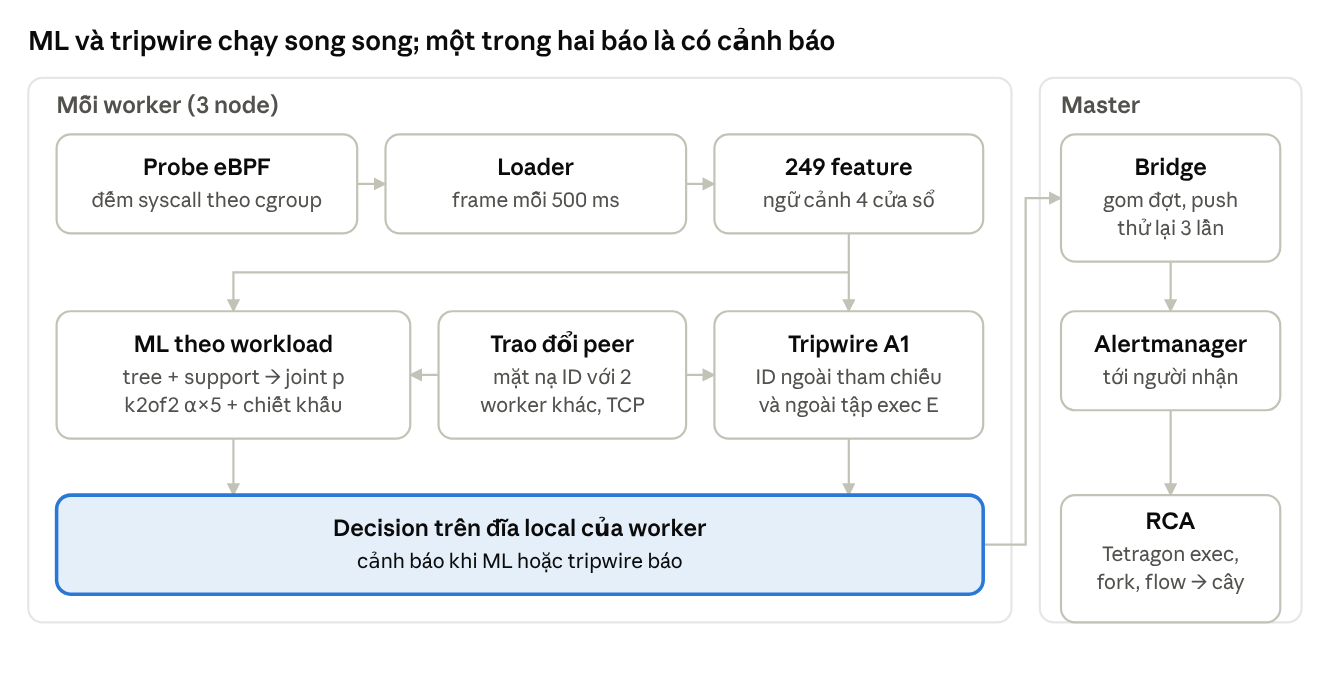
\includegraphics[width=\linewidth]{architecture.png}
  \caption{Kiến trúc Sentinel Pulse (hệ thống cuối, lượt \texttt{pulse-\allowbreak{}final-\allowbreak{}system-\allowbreak{}confirm}).}
  \label{fig:architecture}
\end{figure}

Trên mỗi worker, ML và tripwire cùng đọc một luồng feature và cùng dùng kênh trao đổi với hai worker còn lại. Master chỉ đọc decision đã ghi, đẩy cảnh báo vào Alertmanager, rồi dựng case RCA từ những cảnh báo Alertmanager đã nhận.

\section{Mô hình đe dọa}

\begin{itemize}
\tightlist
\item
  \textbf{Kẻ tấn công} đã chạy được code bên trong một container ứng dụng, tức giai đoạn \emph{sau khi xâm nhập}. Họ khởi chạy một process mới và thử các thao tác ở mức syscall: đổi namespace, ptrace, exec bất thường, đổi quyền vùng nhớ, gọi API seccomp.
\item
  \textbf{Phạm vi được bảo vệ} là mọi replica của 21 workload trong namespace \texttt{production}. Pod hạ tầng, pod tạo tải và các master không được chấm điểm.
\item
  \textbf{Giả thiết tin cậy:} kernel, eBPF, Tetragon và worker của Pulse chưa bị chiếm. Dữ liệu normal dùng để fit và hiệu chỉnh không chứa tấn công.
\item
  \textbf{Ngoài phạm vi:}

  \begin{itemize}
  \tightlist
  \item
    xâm nhập ban đầu qua chính ứng dụng, ví dụ SQL injection hay command injection;
  \item
    tấn công chạy đồng thời trên mọi replica;
  \item
    kẻ tấn công thích nghi chỉ dùng syscall đã có trong hồ sơ normal;
  \item
    tấn công vào host hay hạ tầng cụm.
  \end{itemize}
\end{itemize}

Độ phủ theo MITRE ATT\&CK for Containers chỉ có một phần ở các chiến thuật execution, privilege escalation và defense impairment. Chương 7 bàn về hệ quả của giới hạn này.

\section{Biểu diễn: 249 feature mỗi cửa sổ}

Cứ 0,5 s, user space đọc map eBPF và lấy hiệu số bộ đếm giữa hai lần đọc cho từng cgroup. Vector của một cửa sổ gồm:

\begin{longtable}[]{@{}>{\raggedright\arraybackslash}p{\dimexpr 0.223\linewidth-2\tabcolsep\relax}>{\raggedright\arraybackslash}p{\dimexpr 0.132\linewidth-2\tabcolsep\relax}>{\raggedright\arraybackslash}p{\dimexpr 0.645\linewidth-2\tabcolsep\relax}@{}}
\toprule\noalign{}
Nhóm & Số feature & Nội dung \\
\midrule\noalign{}
\endhead
\bottomrule\noalign{}
\endlastfoot
Syscall tường minh & 58 & log-count và tỉ lệ của 29 syscall (bộ \texttt{base29}) \\
Tổng hợp & 5 & log-count và tỉ lệ của syscall còn lại, log tổng, tỉ lệ syscall nhạy cảm, số lần seccomp từ chối \\
Bin băm syscall & 64 & mọi ID syscall, băm vào 64 bin \\
Bin băm cặp syscall & 64 & cặp syscall liền nhau của cùng thread (cách nhau ≤ 5 s), băm vào 64 bin \\
Trượt 10 cửa sổ & 58 & trung bình và độ lệch chuẩn của 29 syscall trên 10 cửa sổ gần nhất \\
\end{longtable}

Bộ \texttt{base29} gồm:

\begin{itemize}
\tightlist
\item
  syscall thường gặp: \texttt{read}, \texttt{write}, \texttt{open}, \texttt{openat}, \texttt{close}, \texttt{mmap};
\item
  mạng: \texttt{socket}, \texttt{connect}, \texttt{accept}, \texttt{accept4}, \texttt{sendto}, \texttt{recvfrom}, \texttt{sendmmsg}, \texttt{recvmmsg};
\item
  tạo process: \texttt{clone}, \texttt{clone3}, \texttt{execve}, \texttt{execveat};
\item
  11 syscall nhạy cảm: \texttt{mprotect}, \texttt{chmod}, \texttt{ptrace}, \texttt{setuid}, \texttt{setgid}, \texttt{capset}, \texttt{pivot\_\allowbreak{}root}, \texttt{mount}, \texttt{unshare}, \texttt{setns}, \texttt{seccomp}.
\end{itemize}

Nhiều syscall nhạy cảm bằng 0 trên toàn bộ normal. Chính vì vậy chúng là tín hiệu tấn công mà không làm tăng báo nhầm.

Model nhận \textbf{ngữ cảnh} gồm 3 cửa sổ trước và cửa sổ hiện tại, tức 996 số. Hai snapshot cách nhau ngoài 0,35--0,8 s là một \emph{cadence gap}: lịch sử bị xóa và các cửa sổ ngay sau đó không được tính là normal. Mục 6.5 trình bày bằng chứng cho từng nhóm feature.

\section{Model theo workload}

Mỗi workload có một model riêng gồm hai nhánh:

\begin{itemize}
\tightlist
\item
  \textbf{Nhánh tree:} ExtraTrees (\citealp{geurts2006}) học phân biệt ngữ cảnh normal với ngữ cảnh normal bị làm hỏng có chủ đích. Nó nắm được quan hệ giữa lịch sử và cửa sổ hiện tại.
\item
  \textbf{Nhánh support:} với từng feature của cửa sổ hiện tại, lưu vùng giá trị đã thấy khi normal. Điểm là mức vượt ra ngoài vùng đó lớn nhất, chia theo thang của feature. Nhánh này bắt ngay một syscall chưa từng xuất hiện.
\end{itemize}

Mỗi nhánh cho một p-value conformal trên tập calibration riêng, rồi hai p-value được gộp thành joint p (mục 2.4). Ngân sách thiết kế là α = 0,05/30 ≈ 0,00167 mỗi cửa sổ, tức 5\% cho khoảng 15 s. Đây là ngân sách thiết kế dưới giả thiết hoán đổi, không phải bảo đảm.

Calibration được làm mới bằng normal gần nhất trước mỗi lượt live, còn estimator thì giữ nguyên. Model bundle, chính sách và 13 file code chấm điểm đều được khóa bằng SHA-256. Worker từ chối chạy nếu bất kỳ file nào khác bản đóng băng.

\section{Chính sách quyết định: k2of2 α×5 với chiết khấu theo replica}

Một cửa sổ \textbf{đạt} khi thỏa cả hai điều kiện:

\begin{enumerate}
\def\labelenumi{\arabic{enumi}.}
\tightlist
\item
  joint p ≤ 5α (khoảng 0,0083);
\item
  cửa sổ còn mang bằng chứng sau chiết khấu.
\end{enumerate}

Cảnh báo bật khi hai cửa sổ liên tiếp (cách nhau tối đa 1 s) cùng đạt.

\textbf{Chiết khấu theo replica} (chính sách \texttt{policy-\allowbreak{}k2of2-\allowbreak{}a5-\allowbreak{}peer30}) dựa trên một quan sát: phần lớn cảnh báo trên normal đến từ hành vi mà mọi replica của workload đều có, như probe của Kubernetes hay tác vụ định kỳ.

\begin{itemize}
\tightlist
\item
  Mỗi worker phát mặt nạ ID syscall của từng cửa sổ cho các worker khác qua TCP.
\item
  Một cửa sổ \textbf{không còn bằng chứng} khi ngữ cảnh 4 cửa sổ của nó không chứa ID syscall nào mà các replica khác chưa thấy trong 30 s.
\item
  Workload chỉ có một replica, hoặc không có cửa sổ của peer trong 30 s, thì không bao giờ bị chiết khấu.
\end{itemize}

Thiết kế hỏng theo một phía: mất tin của peer chỉ làm bớt chiết khấu, nên detector báo nhiều hơn, không bao giờ ít hơn.

Giới hạn đã đăng ký trước: một tấn công chạy cùng lúc trên mọi replica sẽ bị chiết khấu mất.

\section{Luật tripwire A1}

Tripwire báo khi một cửa sổ chứa ID syscall nằm ngoài cả hai tập sau:

\begin{itemize}
\tightlist
\item
  \textbf{Tham chiếu của workload:} hợp các ID syscall thấy ở mọi replica trong 90 phút đầu của lượt chạy (pha chọn).
\item
  \textbf{Tập exec E:} 59 ID mà việc khởi chạy một binary bất kỳ gây ra. Tập này đóng băng bằng SHA-256.
\end{itemize}

Tham chiếu đến từ cả ba worker qua cùng kênh trao đổi với chiết khấu. Việc chấm bắt đầu 60 s sau khi pha chọn kết thúc, để các cửa sổ tham chiếu đến muộn vẫn được tính.

Tripwire là phiên bản phát hiện của allowlist syscall (mục 3.4):

\begin{itemize}
\tightlist
\item
  nó bắt các hành vi \emph{buộc} phải dùng syscall lạ (\texttt{ptrace}, \texttt{setns}, \texttt{execveat});
\item
  nó không bắt \texttt{mprotect} hay \texttt{seccomp}, vì hai syscall này có sẵn trong hồ sơ normal của nhiều workload.
\end{itemize}

\section{Hệ thống cuối}

Hệ thống cuối báo khi ML \textbf{hoặc} tripwire báo. Tripwire không sửa bất kỳ trường nào của ML, nên các chỉ số của ML vẫn đo riêng được trên cùng lượt chạy.

Cấu hình này được chọn sau khi so sánh có và không có luật (mục 6.6): trong các cách gắn luật đã thử, đây là cách duy nhất giữ mọi chỉ số của ML ở mức ≤ 3 s, đồng thời làm p95 nhanh hơn.

\section{Truy nguyên nguyên nhân (RCA)}

Pulse chỉ cho biết container nào bất thường. RCA trả lời ba câu hỏi tiếp theo: process nào đang chạy, nó đã làm gì, và process nào nên điều tra trước.

\begin{itemize}
\tightlist
\item
  \textbf{Nguồn sự kiện:} ba policy Tetragon chỉ quan sát trong \texttt{production}:

  \begin{itemize}
  \tightlist
  \item
    \texttt{runtime}: file nhạy cảm, credential, kết nối, namespace, ptrace;
  \item
    \texttt{fork};
  \item
    \texttt{flow}: lần gửi trên socket đã mở, lấy mẫu 1 lần mỗi process mỗi 10 s, vì các service dùng connection pool nên hiếm khi gọi \texttt{connect()}.
  \end{itemize}
\item
  \textbf{Ghép:} theo node, Pod UID, container và thời gian, không chỉ theo PID hay IP. Process được định danh bằng \texttt{exec\_\allowbreak{}id} vì PID bị tái sử dụng. Sự kiện được giữ trong một ring 180 s; case lấy 30 s trước cảnh báo.
\item
  \textbf{Gom case:} các cảnh báo cùng container trong 300 s đi vào một case. Trong khoảng đó, nếu container chạy một binary \emph{mới} thì mở thêm case tiếp nối. Binary mới là binary không chạy trong 300 s trước case trước, tra trong nhật ký exec 15 phút.
\item
  \textbf{Xếp hạng nghi phạm:} heuristic có lý do rõ ràng, không phải xác suất.
\end{itemize}

\begin{longtable}[]{@{}>{\raggedright\arraybackslash}p{\dimexpr 0.758\linewidth-2\tabcolsep\relax}>{\raggedright\arraybackslash}p{\dimexpr 0.242\linewidth-2\tabcolsep\relax}@{}}
\toprule\noalign{}
Lý do & Điểm \\
\midrule\noalign{}
\endhead
\bottomrule\noalign{}
\endlastfoot
Binary thấy lần đầu trong workload sau mốc đóng băng baseline & 4 \\
Thao tác credential, namespace, mount, ptrace & 3 mỗi lần, tối đa 9 \\
Binary chưa từng ghi nhận & 2 \\
Exec trong cửa sổ cảnh báo & 2 \\
Syscall thất bại & 1 mỗi lần, tối đa 3 \\
Là cha của một nghi phạm khác & 1 \\
\end{longtable}

Bảng điểm có thêm hai ngoại lệ:

\begin{itemize}
\tightlist
\item
  \texttt{setuid}/\texttt{setgid} hạ xuống ID khác 0 ngay sau khi process khởi động không được tính là thao tác bảo mật. Đây là \emph{luật hạ quyền}: nhiều probe hợp lệ hạ quyền lúc khởi chạy.
\item
  Tiến trình của container runtime (\texttt{containerd-\allowbreak{}shim}, \texttt{runc}) không được xếp hạng.
\end{itemize}

Cây bằng chứng cho thấy liên quan theo định danh và thời gian, không chứng minh nhân quả. RCA cũng không tự xử lý pod.

\section{Đường cảnh báo}

\begin{itemize}
\tightlist
\item
  Một bridge chỉ đọc bám luồng decision trên đĩa local của từng worker và gom các cửa sổ báo thành đợt.
\item
  Mỗi đợt được đẩy thẳng vào Alertmanager của cụm qua API v2. Push lỗi được thử lại 3 lần.
\item
  RCA dựng case từ chính các cảnh báo Alertmanager đã nhận, nên mã đợt cảnh báo và mã case là một.
\end{itemize}

Pulse không dùng đường Prometheus kéo theo chu kỳ. Mục 6.8 cho thấy đường đó chậm hơn nhiều.

\chapter{Cài đặt}

Pulse chạy trên cụm Kubernetes 6 node của phòng lab. Mỗi worker có một loader eBPF viết bằng C và một worker Python chấm điểm. Bridge cảnh báo và RCA chạy trên master đầu tiên. Code, protocol và biên nhận nằm trong cùng một repo git.

\section{Cụm thử nghiệm}

\begin{longtable}[]{@{}>{\raggedright\arraybackslash}p{\dimexpr 0.271\linewidth-2\tabcolsep\relax}>{\raggedright\arraybackslash}p{\dimexpr 0.729\linewidth-2\tabcolsep\relax}@{}}
\toprule\noalign{}
Thành phần & Cấu hình \\
\midrule\noalign{}
\endhead
\bottomrule\noalign{}
\endlastfoot
Node & 3 master (control plane), 3 worker; VM trên ESXi \\
Phần mềm & Kubernetes v1.34.10, Ubuntu 24.04, kernel 6.8.0, Cilium, Istio ambient \\
Ứng dụng & AIMS (An Internet Media Store): frontend, API gateway, các service Python, PostgreSQL (CloudNativePG), Kafka, RabbitMQ, Redis, MinIO; 21 workload, khoảng 80 pod \\
Tải normal & Bốn generator trong namespace \texttt{production}, chuyển qua các chế độ steady, toolmix, peak, burst, recovery theo lịch đăng ký \\
Công cụ runtime có sẵn & Tetragon (nguồn sự kiện cho RCA), Falco (baseline luật) \\
Lưu trữ & NFS riêng cho dữ liệu các lượt chạy \\
\end{longtable}

\section{Thu thập trong kernel}

\begin{itemize}
\tightlist
\item
  \textbf{Loader eBPF} (\texttt{pulse\_\allowbreak{}counter\_\allowbreak{}extended}) gắn chương trình vào \texttt{raw\_\allowbreak{}tp/\allowbreak{}sys\_\allowbreak{}enter} và \texttt{fexit/\allowbreak{}\_\allowbreak{}\_\allowbreak{}seccomp\_\allowbreak{}filter}. Nhờ vậy nó đếm cả syscall bị seccomp từ chối.
\item
  \textbf{Map theo cgroup} giữ ba loại bộ đếm: số đếm theo từng ID syscall (0--1023), 64 bin ID và 64 bin cặp syscall. Bin cặp dùng syscall trước đó của từng thread, nên kernel phải nhớ syscall cuối của mỗi thread.
\item
  \textbf{Danh sách cgroup cho phép} do dịch vụ resolver ghi. Resolver ánh xạ Pod UID → container → cgroup → phiên bản workload.
\item
  \textbf{Cứ 500 ms,} loader đọc map và in một frame JSON ra stdout. Mỗi frame có bộ đếm tích lũy của mọi cgroup được theo dõi.
\item
  \textbf{Khóa bằng proof:} loader và object được khóa bằng SHA-256 cùng một “proof” gắn với phiên bản kernel. Worker từ chối chạy trên kernel khác.
\end{itemize}

\section{Worker chấm điểm}

Worker (\texttt{pipeline/\allowbreak{}matched\_\allowbreak{}worker.\allowbreak{}py}) chạy như một unit systemd trên mỗi worker, giới hạn 3 core và 3 GB RAM. Mỗi frame đi qua các bước:

\begin{enumerate}
\def\labelenumi{\arabic{enumi}.}
\tightlist
\item
  Kiểm tính toàn vẹn: tổng theo ID phải bằng tổng của probe, và bin băm phải bằng phép chiếu của số đếm theo ID. Frame sai bị ghi vào \texttt{issues} và lịch sử được xóa.
\item
  Tính hiệu số với frame trước, dựng 249 feature và ngữ cảnh 4 cửa sổ.
\item
  Chấm theo batch: gom mọi ngữ cảnh cùng workload trong một frame, tối đa 256 bản ghi.
\item
  Áp chính sách, chiết khấu theo replica và tripwire, rồi ghi decision.
\end{enumerate}

\textbf{Đường chấm nhanh} (\texttt{detector/\allowbreak{}fast\_\allowbreak{}forest.\allowbreak{}py}) làm đúng phép tính của scikit-learn: cộng xác suất của từng cây theo thứ tự, bắt đầu từ số 0 float64, nhưng bỏ phần chi phí Python của mỗi cây.

\begin{itemize}
\tightlist
\item
  Batch đầu tiên của mỗi model được chấm bằng cả hai đường. Chỉ cần lệch một giá trị là model đó quay về đường cũ suốt tiến trình.
\item
  Replay 41.250 dòng feature live qua đường tham chiếu cho 0 dòng lệch.
\item
  CPU của worker giảm từ khoảng 94\% xuống 13--31\% một core.
\end{itemize}

\textbf{Khóa bản đóng băng.} Trước khi chấm, worker so SHA-256 của 13 file code chấm điểm với một snapshot đóng băng, và kiểm hash của model bundle cùng chính sách. Nhờ vậy mọi kết quả live gắn với đúng một phiên bản code.

\section{Trao đổi giữa worker}

Mỗi worker mở một cổng TCP (9479), phát mặt nạ ID syscall của từng cửa sổ và nhận mặt nạ của hai worker còn lại. Tin của peer tới sau khoảng 20 ms, nên bucket mới nhất có thể chưa đủ lúc quyết định.

Cùng kênh này mang cửa sổ tham chiếu cho tripwire. Trong lượt cuối, không cửa sổ tham chiếu nào của peer đến muộn.

\section{Ghi dữ liệu ngoài vòng chấm điểm}

Các lượt đầu ghi feature và decision thẳng lên NFS trong vòng chấm điểm. Mỗi lần NFS chậm là một lần frame bị trễ; có frame trễ tới 31,7 s. Hệ thống cuối sửa theo ba cách:

\begin{itemize}
\tightlist
\item
  \textbf{Ghi nền:} mỗi file chia sẻ được ghi qua một hàng đợi và thread riêng. Thread này \texttt{fdatasync} và bỏ page cache mỗi 30 s.
\item
  \textbf{Bản decision trên đĩa local} của worker cho bridge, RCA và campaign đọc.
\item
  \textbf{Trạng thái ghi không đồng bộ.}
\end{itemize}

Kết quả ở lượt cuối:

\begin{itemize}
\tightlist
\item
  độ trễ frame lớn nhất còn 2,4 s;
\item
  lần ghi nền lâu nhất 35 ms, không lần nào phải chờ hàng đợi;
\item
  số lần cách nhịp còn 4, 2 và 1 trên ba worker, so với 8--10 ở lượt trước.
\end{itemize}

\section{Bridge và RCA}

\begin{itemize}
\tightlist
\item
  \textbf{Bridge cảnh báo} chạy trên master, bám file decision local của ba worker và đẩy đợt cảnh báo vào Alertmanager. Ở lượt cuối có 3 push lỗi, cả 3 được thử lại thành công; 5.840/5.840 đợt tới nơi.
\item
  \textbf{Subscriber RCA} đọc luồng sự kiện Tetragon của ba worker vào ring SQLite local, dựng case theo nhịp 0,25 s và giữ tối đa 20.000 case.

  \begin{itemize}
  \tightlist
  \item
    Luồng \texttt{tetra\ getevents} được xoay vòng có giới hạn thời gian sống.
  \item
    DaemonSet Tetragon chạy với \texttt{shareProcessNamespace} để các process \texttt{timeout} kết thúc được thu dọn. Trước khi sửa có 3.931 process zombie trên ba worker.
  \end{itemize}
\end{itemize}

\section{Calibration tự làm mới trong worker}\label{sec:live-recal}

Calibration của bundle cũ dần theo ngày (mục~\ref{sec:limits-calibration}). Worker vì vậy có thêm một chế độ làm mới theo chu kỳ, \texttt{rolling-\allowbreak{}12-\allowbreak{}1}: mỗi giờ, hai mảng calibration của từng workload được thay bằng điểm của các cửa sổ eligible trong 12 giờ trước, gộp cả ba worker. Đây đúng là chiến lược đã cho kết quả tốt nhất trên soak 48 giờ ở phân tích offline.

\begin{itemize}
\tightlist
\item
  \textbf{Không đổi file chấm điểm:} cả đường chấm thường lẫn đường chấm nhanh đọc hai mảng \texttt{calibration\_scores} và \texttt{support\_calibration} của model ở mỗi lần gọi. Vì vậy chỉ cần thay hai mảng giữa hai frame; estimator, ranh giới support, chính sách và 13 file bị ghim SHA-256 giữ nguyên.
\item
  \textbf{Dữ liệu đi ngoài vòng chấm điểm:} mỗi worker ghi điểm thô của mọi cửa sổ vào một bộ đệm theo giờ trên đĩa local (31 byte mỗi cửa sổ). Một thread nền chép giờ vừa xong lên NFS sau 60 s, rồi sau 300 s đọc 12 giờ của cả ba worker và dựng mảng mới. Vòng chấm điểm chỉ nhận mảng đã dựng và thay vào giữa hai frame.
\item
  \textbf{Ghi vết:} mỗi decision mang số \texttt{calibration\_epoch}; epoch chỉ tăng khi có ít nhất một workload được thay. Workload chưa đủ 1.200 cửa sổ giữ mảng cũ.
\item
  \textbf{Khoảng campaign:} trong lượt đánh giá, các khoảng của campaign được loại khỏi calibration, đúng như bản offline. Hệ thống vận hành thật không biết lúc nào bị tấn công, nên đây là một giới hạn (mục~\ref{sec:limits-calibration}).
\item
  \textbf{Kiểm cài đặt:} một script dựng lại từng calibration đã áp dụng chỉ bằng các thành phần offline, rồi so mọi p-value live dưới epoch đó. Trong lượt smoke 75 phút (29/10), cả ba worker áp dụng epoch 1 cho 21/21 workload; 62.887 dòng decision khớp bản dựng lại 100\%, và kích thước mảng giống nhau trên ba worker.
\end{itemize}

Lượt xác nhận 24 giờ theo protocol \texttt{live-\allowbreak{}recalibration-\allowbreak{}confirmation-\allowbreak{}v1} so nhánh live R với chính các dòng đó tính lại bằng calibration của bundle (F). Luật thắng: gánh thấp hơn ít nhất 10\%, recall không kém quá 2 điểm, control không cao quá 1 điểm và p95 không chậm quá 0,2 s.

\section{Quy trình một lượt live}

\begin{enumerate}
\def\labelenumi{\arabic{enumi}.}
\tightlist
\item
  \textbf{Planner} tạo một file \texttt{CONFIG.\allowbreak{}json} bất biến. File này chứa hash của model, chính sách và fixture, lịch tải, lịch trial đã xáo trộn bằng seed cố định, và cấu hình từng worker.
\item
  \textbf{Launcher} cài worker lên ba node, khởi động RCA và bridge, rồi đến traffic và campaign.
\item
  \textbf{90 phút đầu là pha chọn:} tham chiếu của tripwire và baseline binary của RCA được dựng ra rồi đóng băng. Tấn công chỉ bắt đầu sau mốc này 120 s.
\item
  \textbf{Sau khi capture kết thúc,} một chuỗi phân tích tự chạy theo protocol đã commit. Biên nhận JSON được chép vào repo.
\end{enumerate}

Không job nặng nào chạy cùng lúc với lượt live, để điều kiện đo không đổi giữa các lượt.

\chapter{Đánh giá}

Hệ thống cuối đạt cả bốn kỳ vọng đã đăng ký trên một campaign mới, với p95 1,97 s. Điểm yếu chính là binary vô hại vẫn bị gắn cờ 89,5\%. Chương này đi theo thứ tự các câu hỏi nghiên cứu, sau phần phương pháp.

\section{Phương pháp}

\textbf{Đăng ký trước.} Mỗi lượt live và mỗi phân tích chính có một protocol JSON được commit vào git trước khi đọc bất kỳ dòng dữ liệu nào, ví dụ \texttt{final-\allowbreak{}system-\allowbreak{}confirmation-\allowbreak{}v1} hay \texttt{rule-\allowbreak{}integration-\allowbreak{}v1}. Protocol ghi kỳ vọng, định nghĩa chỉ số, luật chọn và code phân tích. Mọi sửa đổi sau đó là một amendment có giờ và lý do.

Kết quả được chia hai loại:

\begin{itemize}
\tightlist
\item
  \textbf{development:} trên dữ liệu đã nhìn khi phát triển;
\item
  \textbf{blind:} trên campaign mới, chưa dùng để chỉnh gì. Chỉ kết quả blind được dùng để kết luận cuối.
\end{itemize}

\textbf{Thiết kế trial.} Mỗi trial nhắm một replica và gồm ba đoạn 15 s liên tiếp trên cùng container:

\begin{enumerate}
\def\labelenumi{\arabic{enumi}.}
\tightlist
\item
  \textbf{Control idle:} không làm gì.
\item
  \textbf{Binary vô hại:} chạy qua cùng đường \texttt{kubectl\ exec} với tấn công, chỉ gọi \texttt{getpid} lặp lại. Đoạn này đo phần tín hiệu chỉ do có process mới.
\item
  \textbf{Tấn công:} một trong 5 kịch bản, lặp theo tốc độ đăng ký.
\end{enumerate}

\begin{longtable}[]{@{}>{\raggedright\arraybackslash}p{\dimexpr 0.389\linewidth-2\tabcolsep\relax}>{\raggedright\arraybackslash}p{\dimexpr 0.611\linewidth-2\tabcolsep\relax}@{}}
\toprule\noalign{}
Kịch bản & Hành vi \\
\midrule\noalign{}
\endhead
\bottomrule\noalign{}
\endlastfoot
\texttt{child\_\allowbreak{}ptrace\_\allowbreak{}handshake} & process con gọi \texttt{ptrace(PTRACE\_\allowbreak{}TRACEME)} \\
\texttt{invalid\_\allowbreak{}setns\_\allowbreak{}burst} & gọi \texttt{setns} với file descriptor -1, luôn thất bại \\
\texttt{execveat\_\allowbreak{}resolution\_\allowbreak{}probe} & gọi \texttt{execveat} tới một file không tồn tại, luôn thất bại \\
\texttt{anonymous\_\allowbreak{}mprotect\_\allowbreak{}churn} & đổi qua lại quyền đọc và đọc--ghi của một trang nhớ ẩn danh \\
\texttt{seccomp\_\allowbreak{}api\_\allowbreak{}probe} & gọi \texttt{seccomp} với mã thao tác không hợp lệ \\
\end{longtable}

Mọi thao tác chỉ ảnh hưởng chính process, hoặc chắc chắn thất bại trước khi đổi trạng thái của host.

\textbf{Quy mô.} 21 workload × 5 kịch bản × 3 tốc độ (6, 12, 24 lần/s) cho 315 trial của \textbf{tập chính}. Từ lượt thứ tư, campaign thêm tốc độ 1 và 3 lần/s để đo kẻ tấn công chậm, nên có 525 trial. Thứ tự trial được xáo bằng seed cố định, và tấn công chỉ bắt đầu sau pha chọn 90 phút.

\textbf{Chỉ số:}

\begin{itemize}
\tightlist
\item
  \textbf{Recall:} tỉ lệ trial tấn công có cảnh báo trong đoạn tấn công.
\item
  \textbf{Control dương:} tỉ lệ đoạn control idle có cảnh báo.
\item
  \textbf{Precision 1:1:} TP / (TP + control dương), vì mỗi trial có đúng một đoạn tấn công và một đoạn control. Tỉ lệ binary vô hại bị gắn cờ được báo riêng, không tính vào precision.
\item
  \textbf{Độ trễ:} từ sự kiện kernel đầu tiên của tấn công tới cuối cửa sổ cảnh báo đầu tiên. Đường tới người nhận qua Alertmanager được đo riêng ở mục 6.8.
\item
  \textbf{Gánh cảnh báo:} số đợt cảnh báo trên mỗi replica-giờ normal, ngoài các khoảng campaign. Một đợt gồm các cửa sổ báo của cùng container cách nhau dưới 15 s.
\end{itemize}

Khoảng tin cậy 95\% dùng Wilson cho tỉ lệ và bootstrap theo workload (10.000 lần) cho gánh cảnh báo và hiệu giữa hai cấu hình.

Có hai cách đếm dùng song song, chênh nhau vài trial:

\begin{itemize}
\tightlist
\item
  \textbf{cách của bộ điều phối campaign:} đếm tới lúc preview được ghi, ví dụ 308/310;
\item
  \textbf{cách so sánh các nhánh:} đếm trên bảng cửa sổ chung của mọi nhánh, ví dụ 313/315.
\end{itemize}

Mỗi bảng dưới đây ghi rõ nó dùng cách nào.

\textbf{Nhãn.} Nhãn là nhãn kỳ vọng theo thiết kế trial. 4.766 cảnh báo trên normal đã được review và không case nào có dấu hiệu độc hại, nhưng người review không độc lập với người thiết kế.

\section{RQ1: sáu lượt live}

\begingroup\footnotesize
\begin{longtable}[]{@{}>{\raggedright\arraybackslash}p{\dimexpr 0.233\linewidth-2\tabcolsep\relax}>{\raggedright\arraybackslash}p{\dimexpr 0.221\linewidth-2\tabcolsep\relax}>{\raggedright\arraybackslash}p{\dimexpr 0.125\linewidth-2\tabcolsep\relax}>{\raggedright\arraybackslash}p{\dimexpr 0.100\linewidth-2\tabcolsep\relax}>{\raggedright\arraybackslash}p{\dimexpr 0.115\linewidth-2\tabcolsep\relax}>{\raggedright\arraybackslash}p{\dimexpr 0.137\linewidth-2\tabcolsep\relax}>{\raggedright\arraybackslash}p{\dimexpr 0.069\linewidth-2\tabcolsep\relax}@{}}
\toprule\noalign{}
Lượt & Luật & Precision & Recall & Control dương & Binary vô hại bị gắn cờ & p95 (s) \\
\midrule\noalign{}
\endhead
\bottomrule\noalign{}
\endlastfoot
pulse-\allowbreak{}live-\allowbreak{}recalibrated & 1 cửa sổ, α×3 & 89,1\% & 92,8\% & 11,2\% & 80,7\% & 1,90 \\
pulse-\allowbreak{}stable-\allowbreak{}candidate & k2of2, α×10 & 92,2\% & 97,8\% & 8,4\% & 92,0\% & 1,85 \\
pulse-\allowbreak{}stable-\allowbreak{}refreshed & k2of2, α×10 + calibration mới & 96,0\% & 100,0\% & 4,2\% & 94,1\% & 2,26 \\
pulse-\allowbreak{}stable-\allowbreak{}confirm & CUSUM b3/h6 \texttt{cap} & 94,6\% & 100,0\% & 5,8\% & 95,1\% & 2,53 \\
pulse-\allowbreak{}peer-\allowbreak{}discount-\allowbreak{}confirm & k2of2 α×5 + chiết khấu replica 30 s & 98,7\% & 98,7\% & 1,3\% & 86,1\% & 2,88 \\
pulse-\allowbreak{}final-\allowbreak{}system-\allowbreak{}confirm (phần ML) & như trên & 99,4\% & 99,4\% & 0,6\% & 89,7\% & 2,38 \\
\end{longtable}
\endgroup

Tập chính, cách đếm của bộ điều phối campaign. Khoảng Wilson của từng ô nằm trong báo cáo kỹ thuật.

Bảng cho thấy ba bước tiến:

\begin{enumerate}
\def\labelenumi{\arabic{enumi}.}
\tightlist
\item
  \textbf{Xác nhận hai cửa sổ (k2of2)} hạ control từ 11,2\% xuống 8,4\% và đưa recall lên 97,8\%.
\item
  \textbf{Làm mới calibration} ngay trước lượt chạy đưa precision lên 96,0\%. Đây là lượt đầu đạt cả bốn kỳ vọng ở mức ≤ 3 s, nhưng gánh còn 6,74 đợt/replica-giờ.
\item
  \textbf{Chiết khấu theo replica} hạ control xuống 1,3\% và gánh xuống 1,69 đợt/replica-giờ.
\end{enumerate}

CUSUM \texttt{cap} không đạt ở lượt xác nhận của nó: control 5,8\% vượt ngưỡng 5\%. Vì vậy nó bị thay theo luật đã đăng ký.

\begin{figure}[htbp]
  \centering
  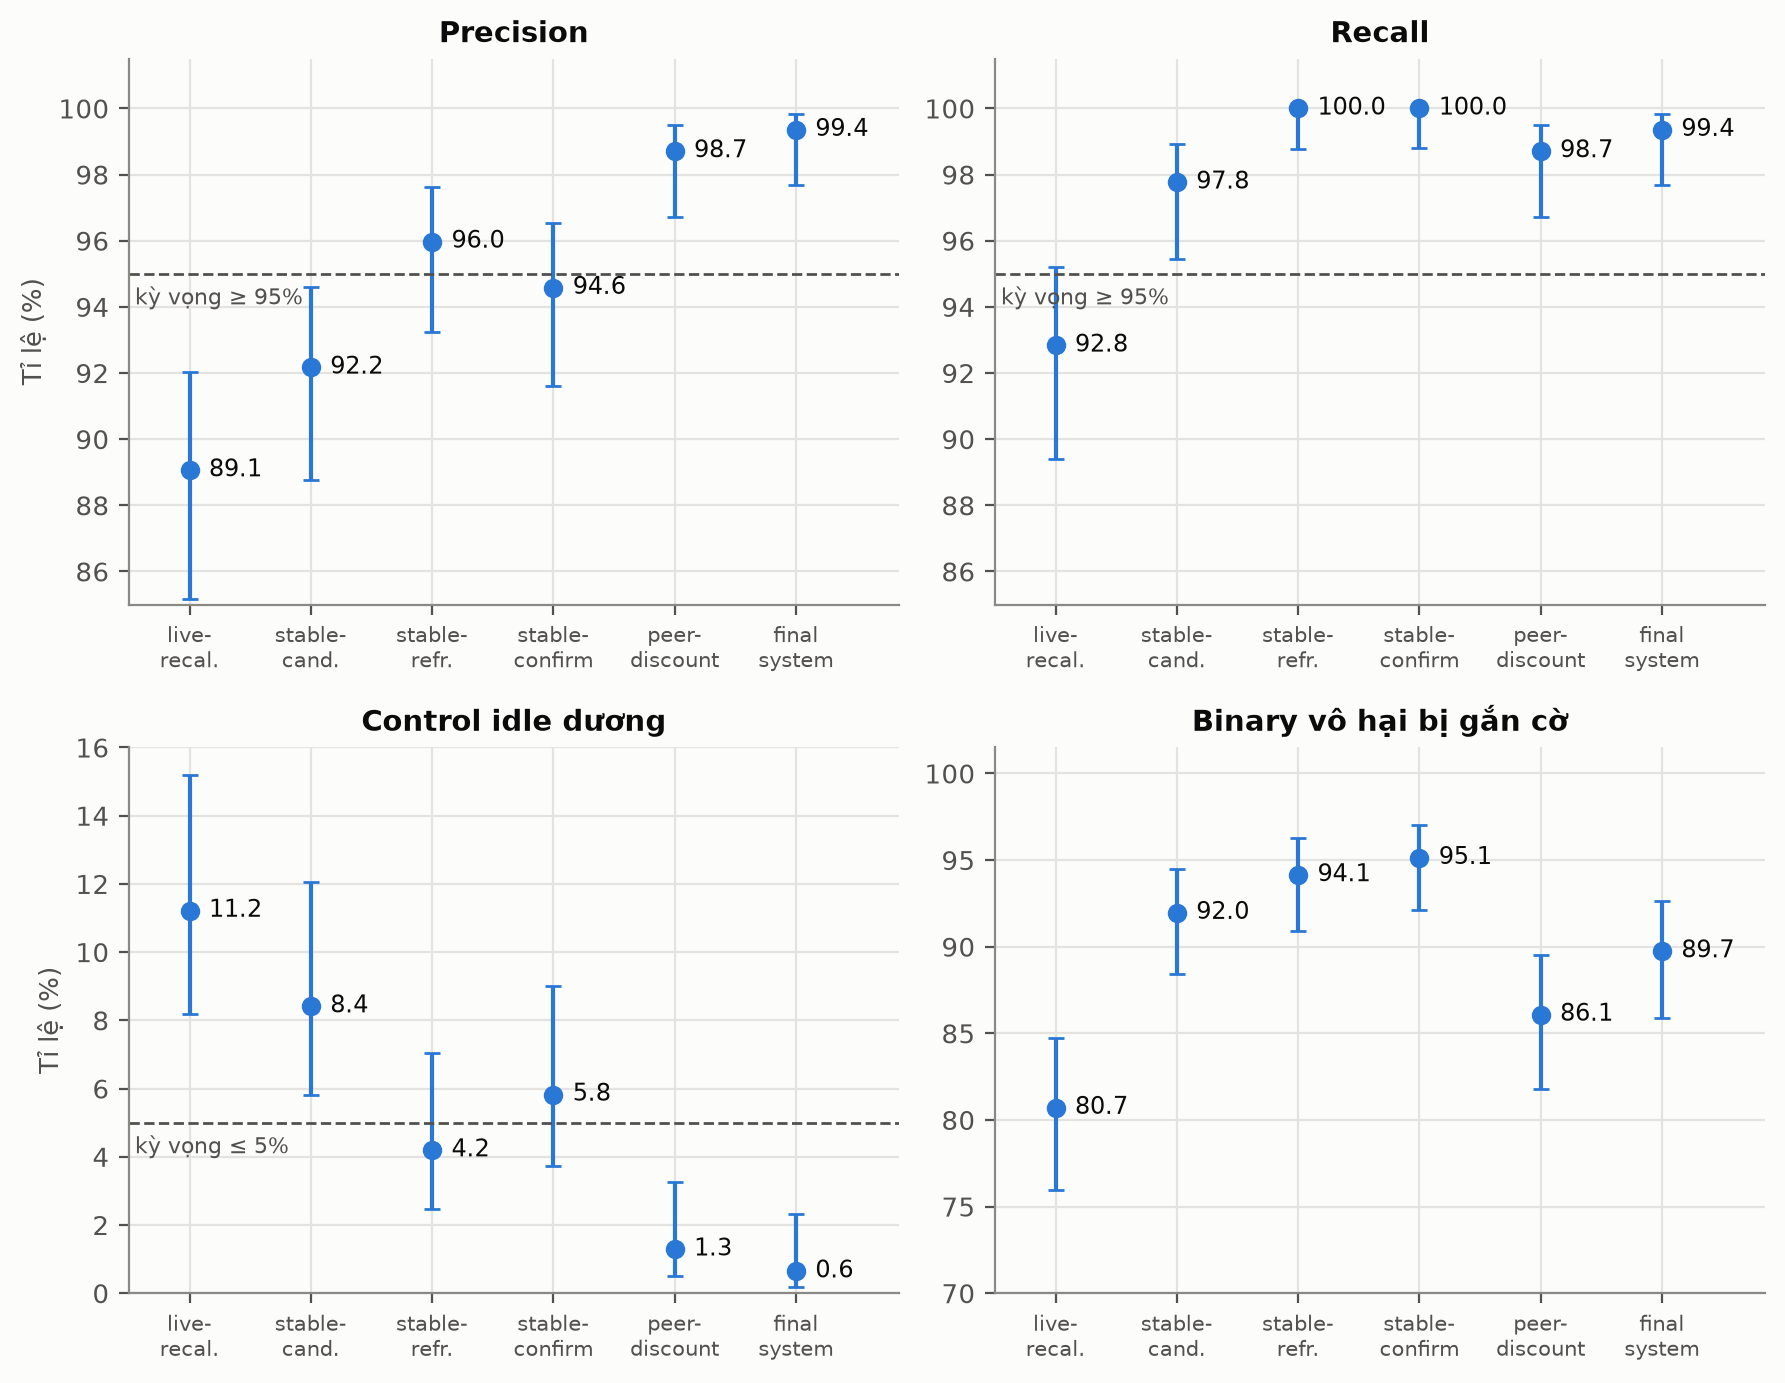
\includegraphics[width=0.85\linewidth]{live-runs-metrics-2x2.png}
  \caption{Precision, recall, control idle dương và binary vô hại bị gắn cờ qua 6 lượt live (phần ML, tập chính), khoảng tin cậy Wilson 95\%. Nhãn kỳ vọng.}
  \label{fig:live-runs-metrics}
\end{figure}

\section{Hệ thống cuối}

Lượt \texttt{pulse-\allowbreak{}final-\allowbreak{}system-\allowbreak{}confirm} chạy từ 25/10 22:05 đến khoảng 22:15 ngày 26/10, với 525 trial. ML được đóng băng từ lượt trước, còn tripwire chạy trong worker.

\begin{longtable}[]{@{}>{\raggedright\arraybackslash}p{\dimexpr 0.396\linewidth-2\tabcolsep\relax}>{\raggedright\arraybackslash}p{\dimexpr 0.198\linewidth-2\tabcolsep\relax}>{\raggedright\arraybackslash}p{\dimexpr 0.309\linewidth-2\tabcolsep\relax}>{\raggedright\arraybackslash}p{\dimexpr 0.097\linewidth-2\tabcolsep\relax}@{}}
\toprule\noalign{}
Chỉ số (tập chính, cách so sánh nhánh) & Kỳ vọng & ML + tripwire {[}CI 95\%{]} & Chỉ ML \\
\midrule\noalign{}
\endhead
\bottomrule\noalign{}
\endlastfoot
Recall & ≥ 95\% & 99,4\% (313/315) {[}97,7; 99,8{]} & 99,4\% \\
Precision & ≥ 95\% & 99,4\% {[}97,7; 99,8{]} & 99,4\% \\
Control dương & ≤ 5\% & 0,6\% (2/314) {[}0,2; 2,3{]} & 0,6\% \\
p95 kernel → cảnh báo đầu tiên & ≤ 3 s, ưu tiên \textless{} 2 s & 1,97 s & 2,25 s \\
Binary vô hại bị gắn cờ & báo kèm & 89,5\% (282/315) & 89,5\% \\
\end{longtable}

Recall, precision và control của hai cột trùng nhau theo định nghĩa, không phải do trùng dữ liệu với lượt khác:

\begin{itemize}
\tightlist
\item
  hệ thống là “ML hoặc tripwire”, nên không bao giờ kém ML;
\item
  ở tập chính, mọi trial mà tripwire bắt thì ML cũng bắt;
\item
  tripwire không gắn cờ control nào và không gắn cờ binary vô hại nào.
\end{itemize}

Tripwire đóng góp ở ba chỗ:

\begin{itemize}
\tightlist
\item
  \textbf{Độ trễ:} p95 nhanh hơn, hiệu nằm trong khoảng 0,02--0,85 s (CI).
\item
  \textbf{Recall trên mọi tốc độ:} tăng từ 93,5\% lên 96,4\%.
\item
  \textbf{Gánh cảnh báo:} trên 849,5 replica-giờ normal, ML có 1,50 đợt/replica-giờ và hệ thống có 1,55. Hiệu +0,049 {[}+0,005; +0,124{]} thấp hơn ngưỡng đăng ký 0,25, nên điều kiện “tripwire thêm rất ít gánh” đạt.
\end{itemize}

Tripwire đứng một mình có recall 60,0\%, vì nó không bắt \texttt{mprotect} và \texttt{seccomp}. P95 của nó là 0,77 s, control 0\%, gánh 0,062 đợt/replica-giờ.

\textbf{Kiểm cài đặt.} Hai bản khớp nhau hoàn toàn:

\begin{itemize}
\tightlist
\item
  tripwire live và tripwire tính lại offline cùng xét 10.417.205 cửa sổ, cùng báo 8.482 cửa sổ, và không lệch cửa sổ nào;
\item
  preview ML live khớp luật tính lại offline ở 99,9999\% cửa sổ.
\end{itemize}

Chênh lệch nhỏ của ML đúng chiều hỏng đã thiết kế: cửa sổ của peer tới muộn thì chiết khấu ít đi, nên live báo nhiều hơn.

\textbf{ML lặp lại.} Theo cách đếm của bộ điều phối, phần ML đạt recall 99,4\% (308/310), precision 99,4\%, control 0,6\% (2/311), p95 2,38 s. Kết quả này xác nhận lại lượt trước trên một campaign mới.

\begin{figure}[htbp]
  \centering
  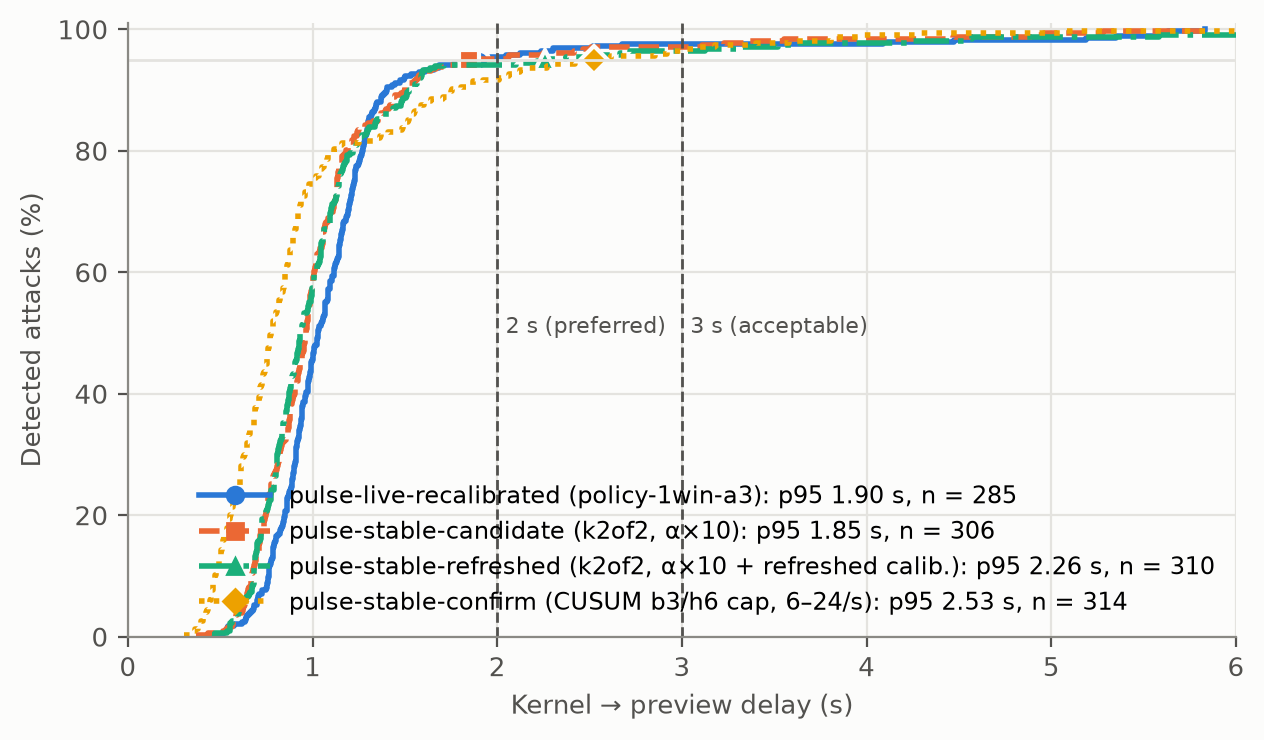
\includegraphics[width=\linewidth]{live-latency-cdf.png}
  \caption{Phân bố độ trễ kernel → preview của các attack được phát hiện, bốn lượt live gần nhất (phần ML, tập chính).}
  \label{fig:live-latency-cdf}
\end{figure}

\section{Kẻ tấn công chậm}

\begin{longtable}[]{@{}ll@{}}
\toprule\noalign{}
Tốc độ (lần/s) & Recall của ML, lượt cuối \\
\midrule\noalign{}
\endhead
\bottomrule\noalign{}
\endlastfoot
1 & 79,0\% (83/105) \\
3 & 90,2\% (92/102) \\
6 & 99,0\% \\
12 & 99,0\% \\
24 & 100\% \\
\end{longtable}

Recall giảm rõ ở 1/s. Chiết khấu theo replica đổi một phần recall ở tấn công chậm lấy control thấp hơn. Ở lượt \texttt{pulse-\allowbreak{}stable-\allowbreak{}confirm}, khi chưa có chiết khấu, recall ở 1/s là 93,1\%. Lý do là cửa sổ của tấn công chậm có ít syscall lạ hơn, nên dễ trùng với hành vi mà các replica khác vẫn có trong 30 s.

\section{RQ2: syscall và nhóm feature nào mang tín hiệu}

Bộ \texttt{base29} được giữ nguyên: không cấu hình thay thế nào tốt hơn có ý nghĩa thống kê. Thí nghiệm fit 11 cấu hình feature đúng như Pulse (21 workload × 11 cấu hình × 3 seed = 693 model). Các cấu hình chỉ khác nhau ở phần syscall tường minh, và được so ở cùng ngân sách cảnh báo với bootstrap theo workload.

\begin{longtable}[]{@{}>{\raggedright\arraybackslash}p{\dimexpr 0.343\linewidth-2\tabcolsep\relax}>{\raggedright\arraybackslash}p{\dimexpr 0.483\linewidth-2\tabcolsep\relax}>{\raggedright\arraybackslash}p{\dimexpr 0.175\linewidth-2\tabcolsep\relax}@{}}
\toprule\noalign{}
Thay đổi so với base29 & Kết quả & Quyết định \\
\midrule\noalign{}
\endhead
\bottomrule\noalign{}
\endlastfoot
Bỏ cặp \texttt{execve}/\texttt{execveat} & Recall −6,7 đến −10,6 điểm, CI loại trừ 0; toàn bộ mức giảm nằm ở kịch bản \texttt{execveat} (100\% xuống 49--66\%) & Giữ \\
Thêm syscall theo tần suất (top-8/16/32) & Không tăng recall; p95 2,9--3,1 s so với 2,3 s & Không thêm \\
Thêm 15 syscall bảo mật hiếm & Chênh recall −0,4 đến +0,3 điểm, CI chứa 0 & Không thêm \\
Mọi ID syscall (\textasciitilde300 feature) & Recall +6--8 điểm ở ngân sách rộng, nhưng binary vô hại bị gắn cờ 96--100\%; p95 5,0 s & Không dùng \\
Bỏ nhánh support & Recall −28,2 {[}−42,5; −15,2{]} điểm; p95 chậm thêm 1,1--1,6 s & Giữ \\
Bỏ nhánh tree & Recall −5,2 {[}−10,6; −1,1{]} điểm ở ngân sách chặt & Giữ \\
Chỉ giữ bin, bỏ kênh syscall tường minh & Recall −13 điểm & Giữ kênh tường minh \\
Bỏ 5 feature tổng hợp & p95 chậm thêm 0,26--0,35 s & Giữ \\
\end{longtable}

Kết luận không đổi khi kiểm lại dưới k2of2 và dưới CUSUM. Bảy syscall hiếm (\texttt{ptrace}, \texttt{setns}, \texttt{execveat}, \texttt{mount}, \texttt{unshare}, \texttt{pivot\_\allowbreak{}root}, \texttt{recvmmsg}) bằng 0 trên 185 triệu lượt gọi normal. Vì vậy chúng mang tín hiệu tấn công mà không làm tăng báo nhầm.

Hai kịch bản dùng syscall phổ biến (\texttt{mprotect}, \texttt{seccomp}) là điểm yếu chung của mọi bộ syscall, với recall 70--83\% ở ngân sách chặt. Đổi bộ syscall không sửa được điểm yếu này.

\textbf{Giới hạn:} đây là kết quả development, và theo luật protocol thì kết quả chính thức là \emph{inconclusive}, vì không cấu hình nào đạt ngân sách 0,1 đợt/giờ. Các so sánh trên được làm ở ngân sách 1, 5 và 18 đợt/giờ.

\begin{figure}[htbp]
  \centering
  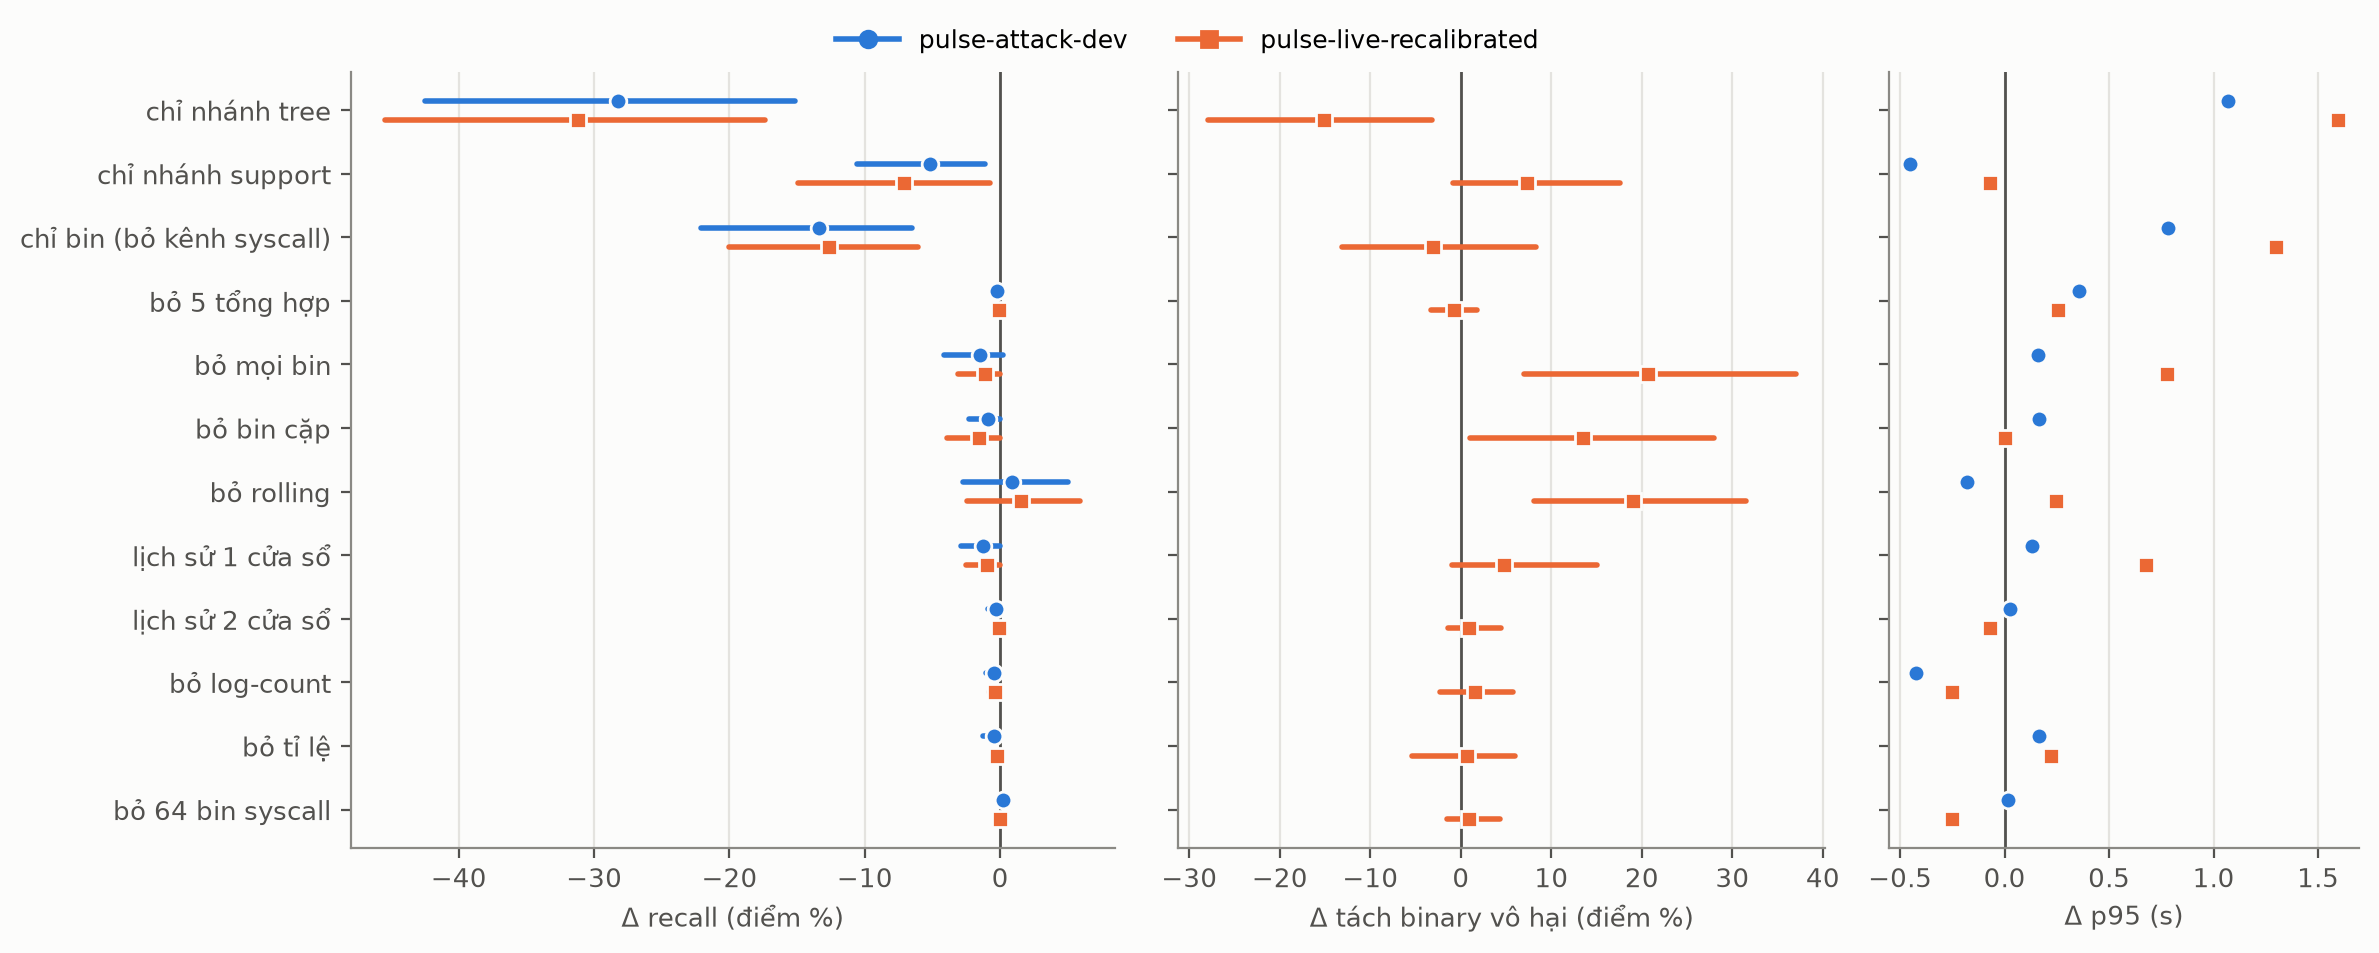
\includegraphics[width=\linewidth]{feature-groups.png}
  \caption{Thay đổi so với base29 khi bỏ một nhóm feature hoặc một nhánh p-value: hiệu recall, hiệu tách binary vô hại (CI bootstrap 95\% theo workload) và hiệu p95. Holdout chính, k2of2, ngân sách 1 (development).}
  \label{fig:feature-groups}
\end{figure}

\section{RQ4: có và không có luật}

Không luật nào tăng recall ở tập chính. ML + tripwire là cách gắn luật duy nhất giữ mọi chỉ số của ML, lại nhanh hơn và gần như không thêm gánh. So sánh chạy trên dữ liệu blind của \texttt{pulse-\allowbreak{}peer-\allowbreak{}discount-\allowbreak{}confirm}, với một khoảng normal chung 706,8 replica-giờ cho mọi nhánh.

\begingroup\footnotesize
\begin{longtable}[]{@{}>{\raggedright\arraybackslash}p{\dimexpr 0.166\linewidth-2\tabcolsep\relax}>{\raggedright\arraybackslash}p{\dimexpr 0.087\linewidth-2\tabcolsep\relax}>{\raggedright\arraybackslash}p{\dimexpr 0.136\linewidth-2\tabcolsep\relax}>{\raggedright\arraybackslash}p{\dimexpr 0.100\linewidth-2\tabcolsep\relax}>{\raggedright\arraybackslash}p{\dimexpr 0.125\linewidth-2\tabcolsep\relax}>{\raggedright\arraybackslash}p{\dimexpr 0.072\linewidth-2\tabcolsep\relax}>{\raggedright\arraybackslash}p{\dimexpr 0.134\linewidth-2\tabcolsep\relax}>{\raggedright\arraybackslash}p{\dimexpr 0.180\linewidth-2\tabcolsep\relax}@{}}
\toprule\noalign{}
Nhánh & Recall & Recall mọi tốc độ & Control & Precision & p95 (s) & Đợt/replica-giờ & Δ đợt so với A {[}CI{]} \\
\midrule\noalign{}
\endhead
\bottomrule\noalign{}
\endlastfoot
A: chỉ ML & 98,7\% & 94,5\% & 1,3\% & 98,7\% & 2,91 & 1,42 & --- \\
B1: ML + Falco & 98,7\% & 95,2\% & 2,9\% & 97,2\% & 2,48 & 2,54 & +1,120 {[}0,000; 3,252{]} \\
B2: ML + tripwire & 98,7\% & 96,6\% & 1,6\% & 98,4\% & 2,44 & 1,48 & +0,066 {[}0,020; 0,133{]} \\
B3: ML rồi lọc probe & 98,7\% & 94,5\% & 1,3\% & 98,7\% & 5,90 & 1,09 & −0,330 {[}−0,751; −0,092{]} \\
Tất cả & 98,7\% & 96,6\% & 3,2\% & 96,9\% & 4,82 & 2,28 & +0,860 {[}−0,409; 3,018{]} \\
\end{longtable}
\endgroup

\begin{itemize}
\tightlist
\item
  \textbf{Falco với bộ luật mặc định} thêm 79\% gánh. Phần thêm này đến từ một luật trên một workload. Nó không tăng recall ở tập chính, vì mọi tấn công ML đều đã bắt.
\item
  \textbf{Lọc probe trước khi gọi người} giảm 23\% gánh, nhưng phải chờ case RCA nên p95 lên 5,90 s, vượt ngưỡng 3 s.
\item
  \textbf{Tripwire} làm p95 nhanh hơn 0,47 s và tăng recall ở tốc độ chậm. Chủ đồ án chọn nhánh này làm hệ thống cuối, và mục 6.3 xác nhận nó trên một lượt live mới.
\end{itemize}

\section{RQ4: tách tấn công khỏi process vô hại mới}

Detector tần suất phát hiện \emph{sự mới lạ}. Qua 6 lượt live, binary vô hại chạy cùng đường exec bị gắn cờ 80,7--95,1\%. Ba baseline cùng khung conformal, cùng k2of2 và cùng ngân sách cho cùng bức tranh (development, ngân sách 1 đợt/replica-giờ):

\begingroup\small
\begin{longtable}[]{@{}>{\raggedright\arraybackslash}p{\dimexpr 0.261\linewidth-2\tabcolsep\relax}>{\raggedright\arraybackslash}p{\dimexpr 0.097\linewidth-2\tabcolsep\relax}>{\raggedright\arraybackslash}p{\dimexpr 0.223\linewidth-2\tabcolsep\relax}>{\raggedright\arraybackslash}p{\dimexpr 0.111\linewidth-2\tabcolsep\relax}>{\raggedright\arraybackslash}p{\dimexpr 0.222\linewidth-2\tabcolsep\relax}>{\raggedright\arraybackslash}p{\dimexpr 0.085\linewidth-2\tabcolsep\relax}@{}}
\toprule\noalign{}
Bộ chấm & Recall & Binary vô hại bị gắn cờ & Control & Tách (recall − vô hại) & p95 (s) \\
\midrule\noalign{}
\endhead
\bottomrule\noalign{}
\endlastfoot
Pulse (base29) & 98,3\% & 79,5\% & 0,6\% & 0,188 & 2,79 \\
Autoencoder & 100\% & 99,3\% & 1,2\% & 0,007 & 1,09 \\
Hồ sơ tần suất kiểu BoSC & 63,1\% & 16,2\% & 1,2\% & 0,469 & 6,25 \\
Isolation Forest & 2,4\% & 1,3\% & 0,6\% & 0,011 & 8,80 \\
\end{longtable}
\endgroup

\begin{itemize}
\tightlist
\item
  \textbf{Autoencoder} bắt tấn công ngang hoặc hơn và nhanh hơn. Ở cùng mức recall 97--98\%, gánh của nó thấp hơn khoảng 9 lần, nhưng nó gắn cờ gần như mọi binary vô hại.
\item
  \textbf{Hồ sơ tần suất} tách binary vô hại tốt nhất, nhưng bỏ sót 37\% tấn công và chậm.
\item
  \textbf{Lặp lại trên dữ liệu mới,} có kiểm định Holm cho 24 so sánh, không baseline nào thay được base29.
\end{itemize}

Hệ quả là đóng góp của Pulse không nằm ở bản thân bộ chấm, mà ở khung đánh giá vận hành và ở tripwire. Tripwire tách được lớp tấn công dùng syscall hiếm: binary vô hại 0\%, còn \texttt{ptrace}, \texttt{setns}, \texttt{execveat} được bắt 100\%.

\begin{figure}[htbp]
  \centering
  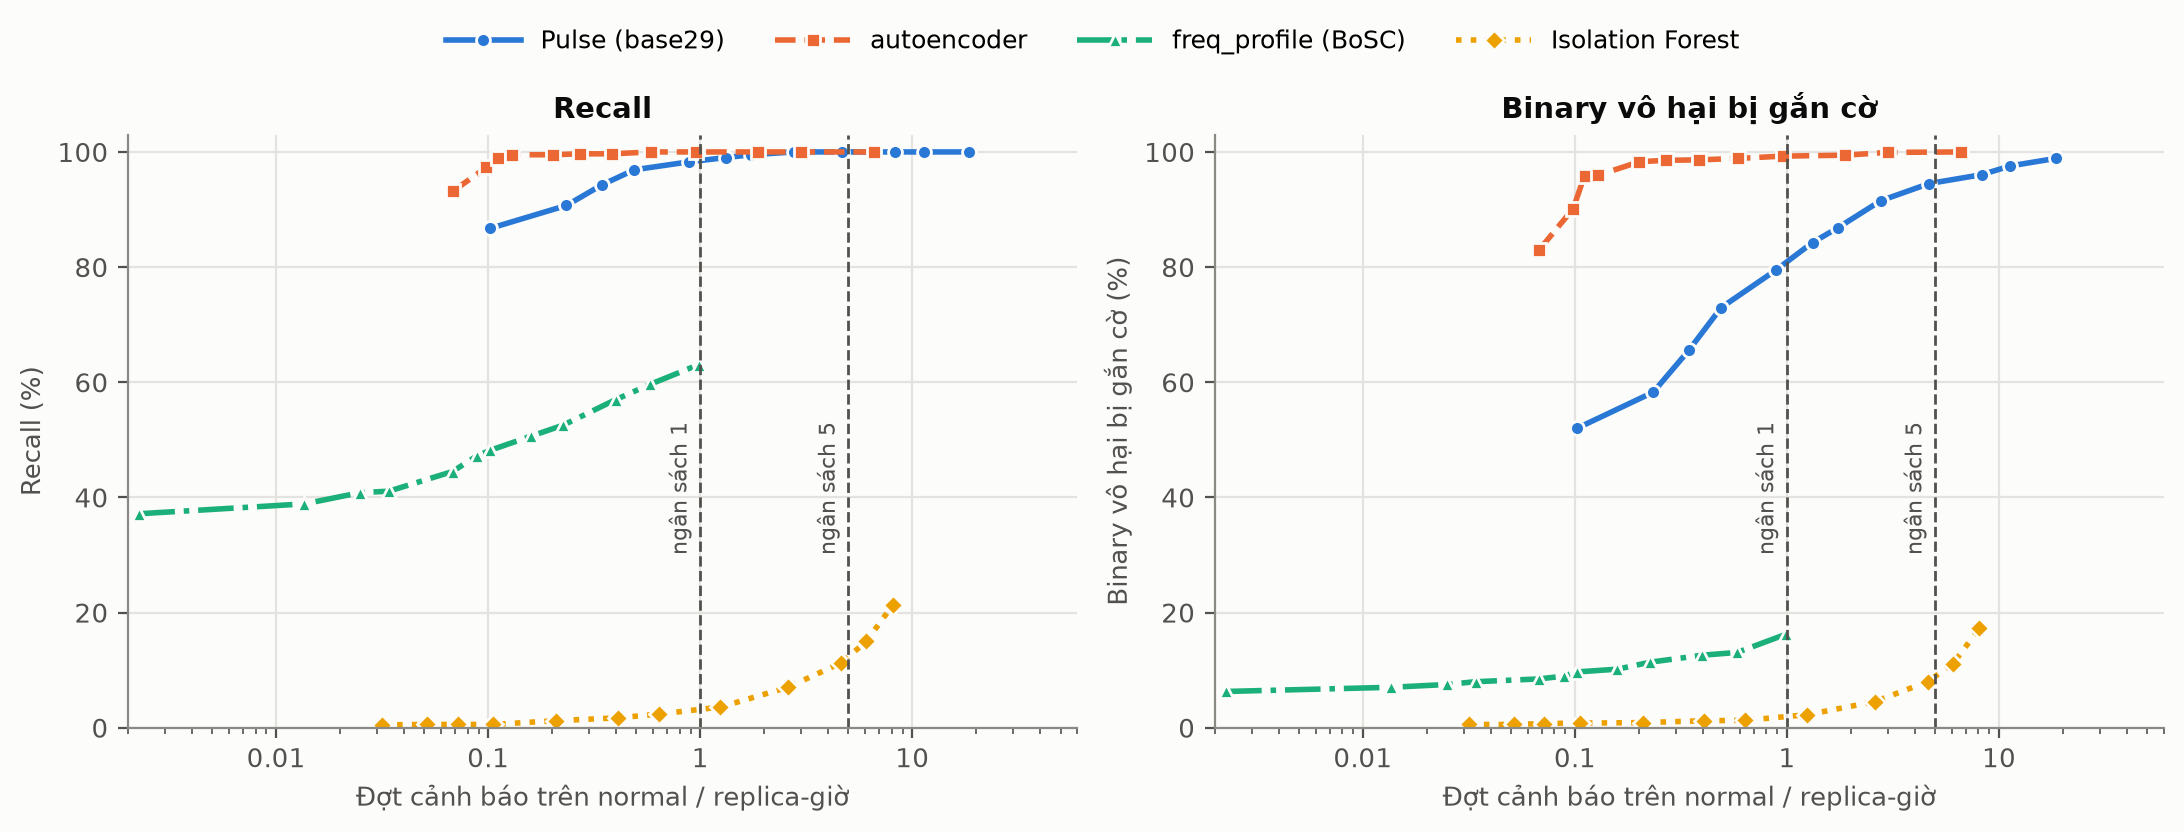
\includegraphics[width=\linewidth]{baselines-budget.png}
  \caption{Recall và tỉ lệ binary vô hại bị gắn cờ theo gánh cảnh báo, Pulse so với ba baseline; mỗi điểm là một hệ số α (development).}
  \label{fig:baselines-budget}
\end{figure}

\section{Đường tới người nhận cảnh báo}

Preview trong decision chưa phải là lúc người vận hành biết. Ở lượt cuối, đường push qua Alertmanager cho 497/525 trial ở mọi tốc độ, tính từ sự kiện kernel tới lúc Alertmanager nhận:

\begin{itemize}
\tightlist
\item
  p50 0,61 s, p95 2,31 s;
\item
  lượt trước, chỉ có ML: p95 3,91 s.
\end{itemize}

Đường Prometheus chuẩn, kéo theo chu kỳ, chậm hơn nhiều: ngay cả với chu kỳ kéo nhanh, p50 đã là 6,4 s. Vì vậy bridge đẩy thẳng là lựa chọn đúng cho mục tiêu dưới 3 s.

\begin{figure}[htbp]
  \centering
  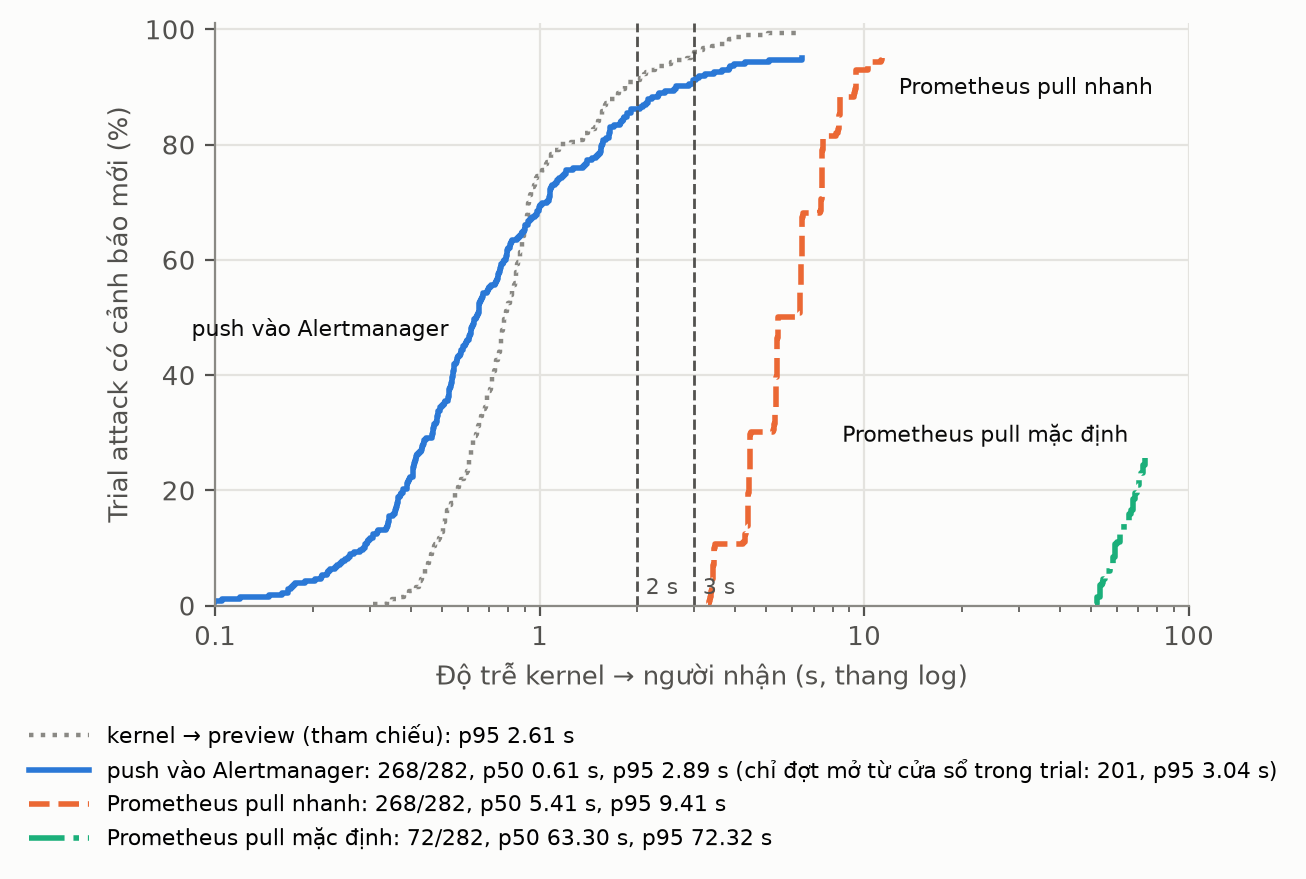
\includegraphics[width=\linewidth]{alert-delivery-cdf.png}
  \caption{Độ trễ kernel → người nhận theo từng đường cảnh báo trên lượt \texttt{pulse-\allowbreak{}stable-\allowbreak{}confirm}: push vào Alertmanager, Prometheus pull nhanh và mặc định.}
  \label{fig:alert-delivery-cdf}
\end{figure}

\section{RQ3: gánh cảnh báo}

Gánh cảnh báo giảm từ 6,74 đợt/replica-giờ xuống 1,50 mà recall vẫn ≥ 95\%, nhưng vẫn gấp khoảng 15 lần ngân sách 0,1. Bốn hướng đã được thử theo protocol đăng ký trước:

\begin{enumerate}
\def\labelenumi{\arabic{enumi}.}
\tightlist
\item
  \textbf{Chỉnh luật dừng (CUSUM, lưới 58 chính sách)} đánh đổi gánh với độ trễ đúng như lý thuyết: siết tham số đưa control về 0,6--2\% nhưng p95 lên 3--5 s.
\item
  \textbf{Chiến lược calibration từ tài liệu} (NexCP, ACI, Mondrian theo node, làm mới theo chu kỳ):

  \begin{itemize}
  \tightlist
  \item
    trên dữ liệu mới, trong 24 giờ sau một lần làm mới, không chiến lược nào thắng;
  \item
    trên soak 48 giờ với calibration đã cũ, làm mới mỗi giờ trên 12 giờ trước giảm 37\% gánh mà không mất recall (development).
  \end{itemize}
\item
  \textbf{Chiết khấu theo replica} đạt test blind (1,74 đợt/replica-giờ, control 2,9\%), rồi được xác nhận live (1,69, bằng 0,37 lần CUSUM).
\item
  \textbf{Lọc probe} giảm gánh nhưng làm chậm đường cảnh báo (mục 6.6).
\end{enumerate}

Cảnh báo còn lại chủ yếu là \emph{benign trigger}:

\begin{itemize}
\tightlist
\item
  57,9\% case trên normal trùng lúc có exec, phần lớn là probe exec của Kubernetes;
\item
  một replica Kafka lệch hệ thống so với hai broker kia và là nguồn gánh lớn nhất.
\end{itemize}

Calibration tự làm mới trong worker (mục~\ref{sec:live-recal}) đã qua smoke với kiểm cài đặt khớp 100\%; lượt xác nhận 24 giờ đang chạy (29--30/10), kết quả sẽ được bổ sung. Lượt này loại khoảng campaign khỏi calibration như bản offline; đây là một giới hạn, vì hệ thống vận hành thật không biết lúc nào bị tấn công.

\begin{figure}[htbp]
  \centering
  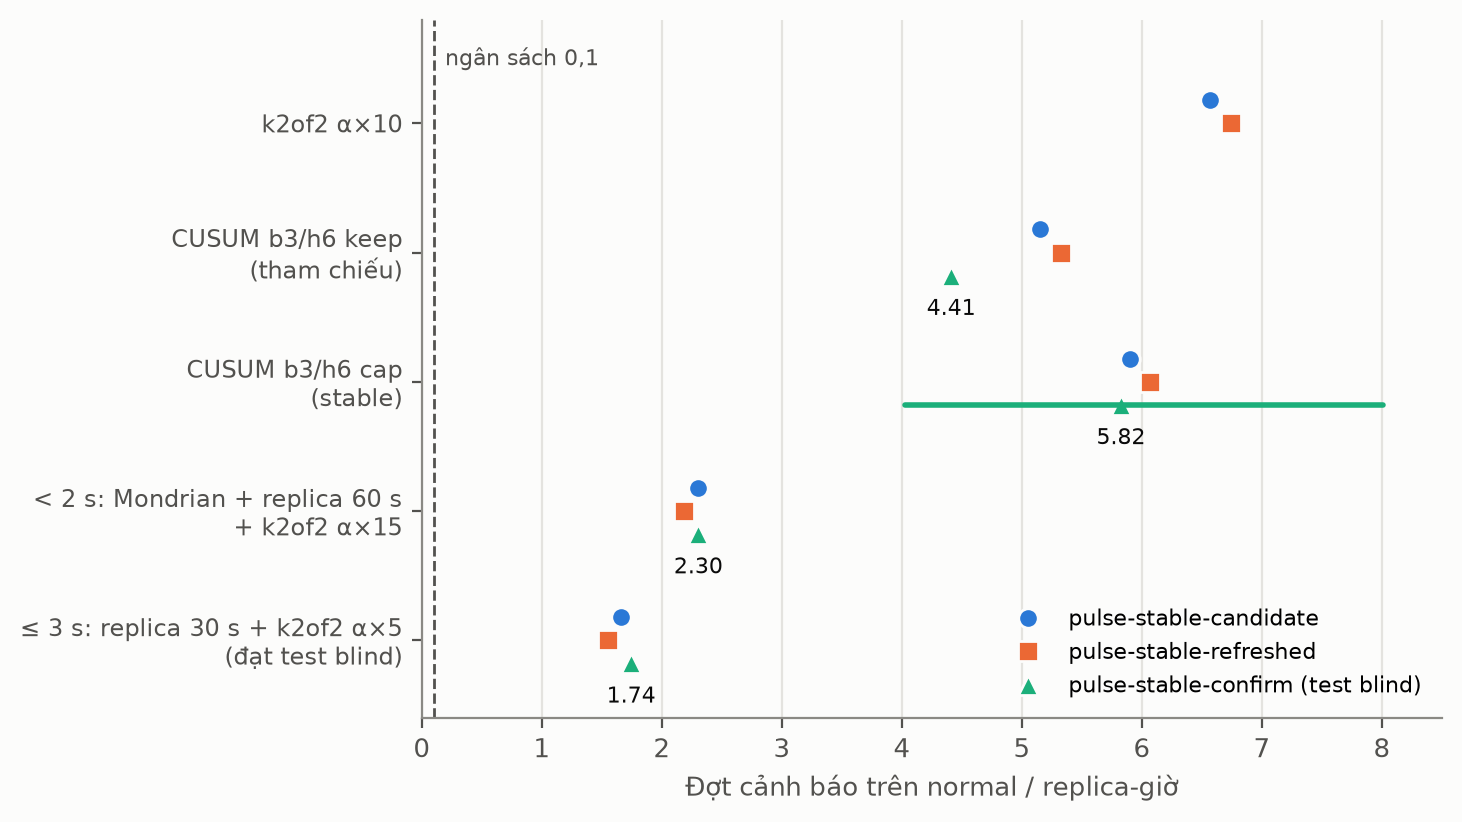
\includegraphics[width=\linewidth]{burden-levers.png}
  \caption{Gánh cảnh báo trên normal (đợt/replica-giờ) của các cấu hình giảm gánh trên hai lượt development và test blind, kèm ngân sách 0,1.}
  \label{fig:burden-levers}
\end{figure}

\section{RQ5: truy nguyên nguyên nhân}

\begingroup\small
\begin{longtable}[]{@{}>{\raggedright\arraybackslash}p{\dimexpr 0.249\linewidth-2\tabcolsep\relax}>{\raggedright\arraybackslash}p{\dimexpr 0.195\linewidth-2\tabcolsep\relax}>{\raggedright\arraybackslash}p{\dimexpr 0.221\linewidth-2\tabcolsep\relax}>{\raggedright\arraybackslash}p{\dimexpr 0.149\linewidth-2\tabcolsep\relax}>{\raggedright\arraybackslash}p{\dimexpr 0.186\linewidth-2\tabcolsep\relax}@{}}
\toprule\noalign{}
Lượt & Tấn công có case riêng & Gộp sau case binary vô hại & Top-1 / top-3 & Cảnh báo → case p95 (s) \\
\midrule\noalign{}
\endhead
\bottomrule\noalign{}
\endlastfoot
pulse-\allowbreak{}stable-\allowbreak{}candidate & 86,7\% (273/315) & 31 & 99,6\% / 99,6\% & 2,52 \\
pulse-\allowbreak{}stable-\allowbreak{}refreshed & 86,7\% (273/315) & 37 & 100\% / 100\% & 2,52 \\
pulse-\allowbreak{}stable-\allowbreak{}confirm & 86,9\% (456/525) & 56 & 99,8\% / 99,8\% & 2,50 \\
pulse-\allowbreak{}peer-\allowbreak{}discount-\allowbreak{}confirm & 87,6\% (459/524) & 44 & 99,8\% / 100\% & 2,59 \\
pulse-\allowbreak{}final-\allowbreak{}system-\allowbreak{}confirm & 89,3\% (469/525) & 40 & 14,1\% / 100\% & 2,67 \\
\end{longtable}
\endgroup

Top-1 là tỉ lệ case có binary tấn công đứng hạng 1 trong danh sách nghi phạm. Top-1 của 4 lượt đầu bị thổi phồng, vì binary vô hại và binary tấn công dùng chung một đường dẫn. Khi binary vô hại có tên riêng ở lượt cuối, nó thường đứng hạng 1 và binary tấn công đứng hạng 2--3:

\begin{itemize}
\tightlist
\item
  top-1 còn 14,1\%, top-3 vẫn 100\%;
\item
  nguyên nhân là luật phá hoà: hai binary thường bằng điểm (6 = binary mới + exec trong cửa sổ), và khi hoà, luật cũ xếp theo thứ tự bảng chữ cái của đường dẫn, nên \texttt{sentinel-\allowbreak{}benign-\allowbreak{}exec-\allowbreak{}control} luôn đứng trước \texttt{sentinel-\allowbreak{}runtime-\allowbreak{}attack-\allowbreak{}blind};
\item
  khi hoà mà xếp process khởi chạy gần cảnh báo nhất lên trước, top-1 trên chính lượt này lên 100\% (469/469). Đây là kết quả development; kiểm blind đã được đăng ký trên lượt kế tiếp. Trong campaign, binary vô hại luôn chạy trước tấn công 15 s, nên luật mới thắng một phần nhờ thiết kế campaign; nó chỉ chứng minh luật cũ là artifact, chưa chứng minh luật mới tốt trong mọi trường hợp.
\end{itemize}

Với 40 tấn công không có case riêng ở lượt cuối, nguyên nhân được quy cho từng bước:

\begin{itemize}
\tightlist
\item
  25 bị từ chối ở bước kiểm exec của case tiếp nối;
\item
  8 không có đợt cảnh báo mới;
\item
  5 có cảnh báo tới chưa đủ 10 s sau case trước;
\item
  2 nằm trong đợt cảnh báo của binary vô hại kéo dài sang.
\end{itemize}

Giả thuyết cho nhóm lớn nhất: khi cảnh báo tới, sự kiện exec của tấn công chưa vào nhật ký exec. Giả thuyết này chưa được kiểm chứng.

\section{RQ6: chi phí}

\textbf{Microbenchmark syscall} trên một worker, ba điều kiện luân phiên, 5 vòng:

\begin{longtable}[]{@{}>{\raggedright\arraybackslash}p{\dimexpr 0.152\linewidth-2\tabcolsep\relax}>{\raggedright\arraybackslash}p{\dimexpr 0.237\linewidth-2\tabcolsep\relax}>{\raggedright\arraybackslash}p{\dimexpr 0.403\linewidth-2\tabcolsep\relax}>{\raggedright\arraybackslash}p{\dimexpr 0.207\linewidth-2\tabcolsep\relax}@{}}
\toprule\noalign{}
Syscall & ns/op khi không có probe & Thêm khi container được theo dõi {[}CI 95\%{]} & ns thêm mỗi syscall \\
\midrule\noalign{}
\endhead
\bottomrule\noalign{}
\endlastfoot
\texttt{getpid} & 1.069 & +24,0\% {[}+17,0; +31,1{]} & \textasciitilde250 \\
\texttt{read} 4 KB & 1.531 & +16,7\% {[}+11,2; +19,2{]} & \textasciitilde253 \\
\texttt{open} + \texttt{close} & 8.134 & +9,4\% {[}+4,6; +17,0{]} & \textasciitilde451 (2 syscall) \\
\texttt{mmap} + \texttt{munmap} & 11.378 & +8,8\% {[}+1,3; +10,5{]} & \textasciitilde400 (2 syscall) \\
\end{longtable}

\begin{itemize}
\tightlist
\item
  Container \textbf{không} được theo dõi vẫn trả khoảng 80--230 ns, vì probe gắn vào \texttt{sys\_\allowbreak{}enter} của cả node rồi mới lọc theo cgroup.
\item
  Mốc không có probe đã cao (\texttt{getpid} khoảng 1,07 µs), nhiều khả năng do VM và các probe khác của cụm. Vì vậy số ns tuyệt đối mới là số so sánh được, không phải phần trăm.
\item
  Worker chấm điểm dùng 13--31\% một core mỗi node.
\end{itemize}

\textbf{Độ trễ request của ứng dụng thật.} Probe làm p95 của request tăng khoảng 3--8\%, nhưng khoảng tin cậy rộng, nên luận văn không nói được rằng mức tăng dưới 5\%. Phép đo theo protocol \texttt{app-\allowbreak{}overhead-\allowbreak{}v1} (cùng amendment 1), đăng ký trước khi đo, chạy ngày 29/10 từ 09:52 đến 11:56:

\begin{itemize}
\tightlist
\item
  hai điều kiện xen kẽ trên cả ba worker: không có probe, và probe của hệ thống cuối gắn đúng như khi live (mọi container \texttt{production} được theo dõi);
\item
  12 vòng, mỗi vòng một block 300 s cho mỗi điều kiện, thứ tự đảo ở vòng chẵn; 30 s đầu của block bị bỏ;
\item
  client mở chạy trên master, 8 request/s, không chờ phản hồi trước; bốn endpoint gọi lần lượt qua ingress Istio, đúng đường người dùng đi; tải normal của AIMS vẫn chạy;
\item
  chỉ số chính: tỉ lệ p95 có probe / không probe của từng endpoint, ghép cặp theo vòng; trung vị qua 12 vòng, CI bootstrap 95\% theo vòng.
\end{itemize}

\begin{longtable}[]{@{}>{\raggedright\arraybackslash}p{\dimexpr 0.25\linewidth-2\tabcolsep\relax}>{\raggedright\arraybackslash}p{\dimexpr 0.19\linewidth-2\tabcolsep\relax}>{\raggedright\arraybackslash}p{\dimexpr 0.19\linewidth-2\tabcolsep\relax}>{\raggedright\arraybackslash}p{\dimexpr 0.2\linewidth-2\tabcolsep\relax}>{\raggedright\arraybackslash}p{\dimexpr 0.17\linewidth-2\tabcolsep\relax}@{}}
\caption{Độ trễ request của AIMS khi có và không có probe (12 vòng, mỗi điều kiện 25.920 request).}\\
\toprule\noalign{}
Endpoint & p95 không probe / có probe (ms) & Thay đổi p95 [CI 95\%] & Thay đổi p50 [CI 95\%] & p50 thêm (ms) \\
\midrule\noalign{}
\endhead
\bottomrule\noalign{}
\endlastfoot
\texttt{/} & 11,5 / 12,1 & +5,9\% [−1,4; +14,5] & +0,5\% [−0,8; +3,2] & 0,04 \\
\texttt{/api/\allowbreak{}health/} & 25,1 / 24,3 & +3,2\% [−8,1; +21,2] & +2,0\% [+0,2; +4,4] & 0,14 \\
\texttt{/api/\allowbreak{}products/} & 306,4 / 318,2 & +8,2\% [+0,7; +18,3] & +3,0\% [+1,2; +4,3] & 5,9 \\
\texttt{/api/\allowbreak{}products/\allowbreak{}?page=1} & 309,3 / 320,4 & +5,8\% [+1,4; +17,9] & +2,6\% [+0,4; +5,2] & 5,3 \\
\end{longtable}

Cột p95 là trung vị qua các vòng của p95 từng block; cột thay đổi là trung vị của tỉ lệ ghép cặp, nên hai cột không suy ra nhau trực tiếp (ở \texttt{/api/\allowbreak{}health/}, trung vị p95 giảm nhưng trung vị tỉ lệ tăng).

\begin{itemize}
\tightlist
\item
  \textbf{Theo luật đã đăng ký,} chỉ được nói ``dưới 5\%'' khi cận trên CI dưới +5\% ở cả bốn endpoint. Cận trên thực tế là +14,5\% đến +21,2\%, nên kết luận ``dưới 5\%'' \emph{không} được đưa ra.
\item
  \textbf{Ở trung vị,} p50 tăng 0,5--3,0\%. Hai lệnh đọc \texttt{/api/\allowbreak{}products/} đi qua nhiều service và cơ sở dữ liệu, nên chậm thêm nhiều nhất: khoảng 5--6 ms ở p50 trên nền khoảng 200 ms. Đây là đường có nhiều syscall nhất trong bốn endpoint, nên hướng của kết quả khớp với chi phí theo từng syscall của microbenchmark.
\item
  \textbf{CPU:} tiến trình loader dùng 0,016--0,041 core mỗi worker. Tính cả phần chạy trong kernel, tỉ lệ CPU bận của node tăng 0,4--0,9 điểm phần trăm, tức khoảng 0,09--0,21 core trên 24 core.
\item
  \textbf{Lỗi:} 0,57\% request lỗi khi không có probe và 0,55\% khi có probe. Phần lớn số lỗi rơi vào một đợt timeout khoảng 60 s ở block đầu tiên, khi chưa gắn probe.
\item
  \textbf{Giới hạn:} phép đo chỉ gồm probe trong kernel và việc đọc map. Scorer ở user space không xen kẽ được theo block 5 phút, vì mỗi lần khởi động cần 90 phút pha chọn; CPU của nó được lấy từ các lượt live (13--31\% một core). Phép đo chạy trên một cụm VM, một kernel.
\end{itemize}

\section{LID-DS 2021}

Trên 15 kịch bản lỗ hổng thật của LID-DS 2021, hệ thống cuối phát hiện 77,3\% bản ghi tấn công và báo nhầm trên 3,0\% bản ghi normal, với mọi tham số lấy nguyên từ hệ thống live. STIDE phát hiện mọi bản ghi tấn công, nhưng báo nhầm trên 60,8\% bản ghi normal.

Đánh giá theo protocol \texttt{lidds-\allowbreak{}evaluation-\allowbreak{}v1}, đăng ký ngày 29/10 lúc 09:17, trước mọi lần fit:

\begin{itemize}
\tightlist
\item
  mỗi kịch bản là một workload; model được fit trên training, hiệu chỉnh trên validation và chỉ đánh giá trên hai tập test, đúng cách chia của dataset;
\item
  trace syscall được chuyển thành đúng các frame mà loader eBPF sinh ra, rồi chạy qua cùng bộ dựng 249 feature;
\item
  quyết định giống live nhưng không có chiết khấu theo replica, vì một bản ghi chỉ có một container;
\item
  một bản ghi tấn công được tính là phát hiện khi có cảnh báo kết thúc sau thời điểm exploit đầu tiên mà LID-DS ghi lại; độ trễ tính từ thời điểm đó; bản ghi normal bị báo nhầm khi có bất kỳ cảnh báo nào;
\item
  baseline STIDE \citep{forrest1996}: cơ sở dữ liệu chuỗi 7 tên syscall theo từng thread trên training; một cửa sổ báo khi có chuỗi không có trong cơ sở dữ liệu; không chỉnh tham số.
\end{itemize}

\begin{longtable}[]{@{}>{\raggedright\arraybackslash}p{\dimexpr 0.25\linewidth-2\tabcolsep\relax}>{\raggedright\arraybackslash}p{\dimexpr 0.24\linewidth-2\tabcolsep\relax}>{\raggedright\arraybackslash}p{\dimexpr 0.24\linewidth-2\tabcolsep\relax}>{\raggedright\arraybackslash}p{\dimexpr 0.12\linewidth-2\tabcolsep\relax}>{\raggedright\arraybackslash}p{\dimexpr 0.15\linewidth-2\tabcolsep\relax}@{}}
\caption{LID-DS 2021, gộp 15 kịch bản: 1.815 bản ghi tấn công, 11.341 bản ghi normal (137,5 giờ normal).}\\
\toprule\noalign{}
Nhánh & Phát hiện [CI 95\%] & Bản ghi normal bị báo nhầm [CI 95\%] & Đợt/giờ normal & Độ trễ p50 / p95 (s) \\
\midrule\noalign{}
\endhead
\bottomrule\noalign{}
\endlastfoot
ML & 63,6\% (1154/1815) [61,3; 65,8] & 2,9\% (333/11341) [2,6; 3,3] & 2,46 & 1,33 / 4,13 \\
Tripwire & 63,5\% (1153/1815) [61,3; 65,7] & 0,1\% (7/11341) [0,0; 0,1] & 0,05 & 0,79 / 2,94 \\
Hệ thống (ML hoặc tripwire) & 77,3\% (1403/1815) [75,3; 79,2] & 3,0\% (336/11341) [2,7; 3,3] & 2,48 & 0,77 / 2,71 \\
STIDE & 100,0\% (1815/1815) [99,8; 100,0] & 60,8\% (6899/11341) [59,9; 61,7] & 59,95 & 0,37 / 1,44 \\
\end{longtable}

Hiệu gộp, bootstrap theo kịch bản (10.000 lần), tính bằng điểm phần trăm:

\begin{itemize}
\tightlist
\item
  hệ thống so với ML: phát hiện +13,7 [+0,2; +30,0], báo nhầm +0,0 [+0,0; +0,1];
\item
  hệ thống so với STIDE: phát hiện -22,7 [-42,1; -6,5], báo nhầm -57,9 [-76,6; -38,9].
\end{itemize}

\begingroup\small
\begin{longtable}[]{@{}>{\raggedright\arraybackslash}p{\dimexpr 0.27\linewidth-2\tabcolsep\relax}>{\raggedright\arraybackslash}p{\dimexpr 0.11\linewidth-2\tabcolsep\relax}>{\raggedright\arraybackslash}p{\dimexpr 0.13\linewidth-2\tabcolsep\relax}>{\raggedright\arraybackslash}p{\dimexpr 0.13\linewidth-2\tabcolsep\relax}>{\raggedright\arraybackslash}p{\dimexpr 0.2\linewidth-2\tabcolsep\relax}>{\raggedright\arraybackslash}p{\dimexpr 0.16\linewidth-2\tabcolsep\relax}@{}}
\caption{LID-DS 2021 theo kịch bản (\%). Báo nhầm là tỉ lệ bản ghi normal có cảnh báo.}\\
\toprule\noalign{}
Kịch bản & ML phát hiện & Tripwire phát hiện & Hệ thống phát hiện & Báo nhầm: hệ thống / STIDE & STIDE phát hiện \\
\midrule\noalign{}
\endhead
\bottomrule\noalign{}
\endlastfoot
\texttt{Bruteforce\_CWE-\allowbreak{}307} & 96,4 & 0,0 & 96,4 & 2,7 / 10,7 & 100,0 \\
\texttt{CVE-\allowbreak{}2012-\allowbreak{}2122} & 100,0 & 100,0 & 100,0 & 1,0 / 36,4 & 100,0 \\
\texttt{CVE-\allowbreak{}2014-\allowbreak{}0160} & 5,8 & 0,0 & 5,8 & 15,6 / 3,0 & 100,0 \\
\texttt{CVE-\allowbreak{}2017-\allowbreak{}12635\_6} & 100,0 & 100,0 & 100,0 & 2,1 / 100,0 & 100,0 \\
\texttt{CVE-\allowbreak{}2017-\allowbreak{}7529} & 69,7 & 0,0 & 69,7 & 1,6 / 15,2 & 100,0 \\
\texttt{CVE-\allowbreak{}2018-\allowbreak{}3760} & 4,1 & 100,0 & 100,0 & 2,6 / 98,6 & 100,0 \\
\texttt{CVE-\allowbreak{}2019-\allowbreak{}5418} & 16,7 & 0,0 & 16,7 & 0,7 / 96,8 & 100,0 \\
\texttt{CVE-\allowbreak{}2020-\allowbreak{}13942} & 98,3 & 100,0 & 100,0 & 1,1 / 99,7 & 100,0 \\
\texttt{CVE-\allowbreak{}2020-\allowbreak{}23839} & 51,7 & 100,0 & 100,0 & 2,5 / 39,7 & 100,0 \\
\texttt{CVE-\allowbreak{}2020-\allowbreak{}9484} & 100,0 & 100,0 & 100,0 & 2,4 / 98,8 & 100,0 \\
\texttt{CWE-\allowbreak{}89-\allowbreak{}SQL-\allowbreak{}injection} & 100,0 & 100,0 & 100,0 & 2,0 / 47,1 & 100,0 \\
\texttt{EPS\_CWE-\allowbreak{}434} & 100,0 & 100,0 & 100,0 & 2,1 / 37,5 & 100,0 \\
\texttt{Juice-\allowbreak{}Shop} & 4,1 & 62,0 & 63,6 & 0,8 / 99,9 & 100,0 \\
\texttt{PHP\_CWE-\allowbreak{}434} & 100,0 & 100,0 & 100,0 & 1,4 / 31,4 & 100,0 \\
\texttt{ZipSlip} & 3,4 & 0,0 & 3,4 & 5,8 / 97,8 & 100,0 \\
\end{longtable}
\endgroup

\begin{itemize}
\tightlist
\item
  \textbf{Mạnh:} hệ thống phát hiện 100\% ở 9/15 kịch bản, với 1,0--2,6\% bản ghi normal bị báo nhầm. Tripwire phát hiện 100\% ở 9 kịch bản và gần như không báo nhầm (0,1\% gộp). Nó bù cho ML ở chỗ ML yếu, ví dụ \texttt{CVE-\allowbreak{}2018-\allowbreak{}3760}: ML 4,1\%, tripwire 100\%.
\item
  \textbf{Yếu:} \texttt{CVE-\allowbreak{}2014-\allowbreak{}0160} (Heartbleed, 5,8\%), \texttt{ZipSlip} (3,4\%), \texttt{CVE-\allowbreak{}2019-\allowbreak{}5418} (16,7\%), \texttt{Juice-\allowbreak{}Shop} (63,6\%, gần như chỉ nhờ tripwire) và \texttt{CVE-\allowbreak{}2017-\allowbreak{}7529} (69,7\%). Ở các kịch bản này, exploit chạy bên trong chính process của dịch vụ. Cách giải thích khả dĩ là exploit không cần syscall mới, cũng không đổi đáng kể tần suất syscall; đây là cách giải thích, chưa được kiểm riêng. Nó khớp với giới hạn ở mục~\ref{sec:limits-novelty}: số đếm syscall yếu với tấn công đi qua ứng dụng.
\item
  \textbf{STIDE} \emph{bắt} mọi bản ghi tấn công, nhưng đổi lại báo nhầm trên 60,8\% bản ghi normal (gần 60 đợt mỗi giờ normal). Biến thể \emph{any-mismatch} không có ngưỡng, và protocol không cho chỉnh tham số sau khi xem kết quả. Vì vậy con số này là của STIDE nguyên bản, không phải của một STIDE đã tinh chỉnh.
\item
  \textbf{Độ trễ:} p95 2,71 s của hệ thống tính từ thời điểm exploit đến cuối cửa sổ cảnh báo, trong điều kiện replay; chưa gồm đường tới người nhận.
\item
  \textbf{Giới hạn đã phát hiện sau khi chạy:} bộ chuyển đổi đã bỏ bốn syscall thật vì sysdig ghi tên khác với bảng ABI: \texttt{pread}, \texttt{pwrite}, \texttt{sigreturn}, \texttt{prlimit}. Tổng cộng khoảng 15 triệu lượt gọi ở 12/15 kịch bản. Lỗi này giống nhau giữa train và test nên không làm rò nhãn, nhưng Pulse thấy ít thông tin hơn STIDE (STIDE đọc tên thô). Bộ chuyển đổi đã được sửa, và một lượt chạy lại đã được đăng ký là phân tích độ nhạy (amendment 1). Bảng trên là kết quả của lượt đã đăng ký.
\item
  \textbf{Đặt cạnh số đã công bố:} kết quả duy nhất trên đủ 15 kịch bản LID-DS 2021 mà tác giả dataset công bố là STIDE (chuỗi 7 syscall, cửa sổ 100 syscall, ngưỡng là điểm cao nhất trên validation), với tỉ lệ phát hiện trung bình 0,59 \citep{grimmer2022}. Hệ thống của luận văn đạt 0,773. Báo nhầm của bài đó được đếm theo số cụm báo động chứ không theo bản ghi, nên chỉ so được tỉ lệ phát hiện. LID-DS chưa có ngưỡng đạt nào được đăng ký.
\item
  \textbf{Lượt v2 đã đăng ký} (protocol \texttt{lidds-\allowbreak{}evaluation-\allowbreak{}v2}): thêm các tín hiệu theo tham số và giá trị trả về (đường dẫn mới, lỗi theo errno, số byte) và chuỗi syscall theo thread, với ngưỡng là điểm cao nhất trên validation. Protocol ghi rõ thiết kế được làm sau khi đã thấy kết quả trên, nên bằng chứng độc lập chỉ đến từ lượt xác nhận trên LID-DS 2019 và CB-DS.
\end{itemize}

\chapter{Thảo luận và giới hạn}

Kết quả mạnh nhất của luận văn là độ trễ và độ tin cậy của việc đo trên cụm thật. Giới hạn lớn nhất là recall đo được chỉ là cận trên cho tấn công đi vào qua exec, và detector chưa phân biệt được ác ý với sự mới lạ.

\section{Detector phát hiện sự mới lạ, không phải ác ý}\label{sec:limits-novelty}

Mọi tấn công trong campaign đều là một process mới chạy qua exec, và Pulse bắt “có process mới” rất mạnh. Hai quan sát cho thấy điều này:

\begin{itemize}
\tightlist
\item
  binary vô hại bị gắn cờ 80,7--95,1\%;
\item
  57,9\% cảnh báo trên normal trùng lúc có exec.
\end{itemize}

Vì vậy recall gần 100\% có thể bị thổi phồng một phần bởi chính dấu hiệu exec. Đây là dạng tương quan giả mà \citet{arp2022} cảnh báo. Đối chứng binary vô hại đo được mức thổi phồng, nhưng không cho biết recall khi tấn công không sinh process mới.

Tripwire tách được một lớp: tấn công buộc phải dùng syscall lạ. Hai kịch bản \texttt{mprotect} và \texttt{seccomp} thì chỉ còn tín hiệu tần suất. Muốn tiến xa hơn cần thông tin ngoài số đếm, ví dụ tham số syscall hay quan hệ cha--con của process (Chương 8).

\section{Gánh cảnh báo}

Gánh 1,50--1,55 đợt/replica-giờ còn gấp khoảng 15 lần ngân sách 0,1. Với khoảng 80 container, con số này tương đương cỡ 2.900 đợt cảnh báo mỗi ngày (ước tính 1,5 × 80 × 24).

Precision 99,4\% đo trên campaign cân bằng 1:1. Ở tỉ lệ tấn công thật, precision sẽ thấp hơn rất nhiều. Vì vậy luận văn báo gánh cảnh báo như một giới hạn, không coi precision là bằng chứng dùng được trong vận hành.

Phần lớn cảnh báo còn lại là benign trigger có cấu trúc, nên có thể xử lý ở tầng sau:

\begin{itemize}
\tightlist
\item
  probe exec của Kubernetes;
\item
  một replica Kafka lệch so với hai broker còn lại.
\end{itemize}

Lọc probe đã giảm 23\% gánh, nhưng phải chờ RCA nên chậm. Calibration riêng theo replica cho Kafka chưa được thử.

Về độ lớn: muốn về ngân sách 0,1 thì phải giảm thêm khoảng 93,5\%. Mức giảm báo nhầm tốt nhất đã công bố bằng cách xếp hạng cảnh báo theo ngữ cảnh, khoảng 84--86\% (\citealp{hassan2019}), vẫn để lại 2--2,5 lần ngân sách. Khoảng cách này là hệ quả của việc đo sự mới lạ, không phải của việc chỉnh tham số. Nghiên cứu về SOC cũng cho thấy phần lớn cảnh báo bị coi là ``sai'' thực ra là benign trigger: hệ thống thấy đúng sự kiện, chỉ là sự kiện vô hại (\citealp{alahmadi2022}). Gom các đợt cảnh báo thành sự cố và tương quan với sự kiện của Kubernetes là đòn bẩy còn lại cho vận hành, nhưng không thay đổi tỉ lệ binary vô hại bị gắn cờ.

\section{Tính thực tế của tấn công}

\begin{itemize}
\tightlist
\item
  \textbf{Giai đoạn:} fixture tự viết mô phỏng giai đoạn sau xâm nhập. Mọi thao tác cố ý thất bại hoặc chỉ ảnh hưởng chính process, kéo dài 15 s, với tốc độ 1--24 lần/s.
\item
  \textbf{Độ phủ ATT\&CK for Containers:} chưa có initial access qua ứng dụng, persistence, credential access, discovery, lateral movement hay impact (ví dụ đào coin).
\item
  \textbf{Tấn công đi qua process của dịch vụ} (SQL injection, command injection) chưa được đo trên cụm.
\item
  \textbf{Exploit thật:} đánh giá trên LID-DS (mục 6.12) bù một phần với 15 kịch bản lỗ hổng thật, nhưng đó là đánh giá offline trên trace ghi sẵn, không phải trên cụm.
\end{itemize}

Về quy mô, campaign của luận văn không nhỏ so với các đánh giá đã công bố: một so sánh gần đây giữa Falco, Tetragon và Tracee dùng 3 tấn công, mỗi tấn công lặp 20 lần, và báo tỉ lệ báo nhầm 0\% mà không mô tả tải vô hại (\citealp{syairozi2025}); ReplicaWatcher dùng 13 kịch bản CVE/CWE trên hai ứng dụng (\citealp{elkhairi2024}). Khoảng trống thật của luận văn không nằm ở số kịch bản mà ở loại kịch bản: chưa có exploit chạy trong chính process của dịch vụ trên cụm, đúng loại mà LID-DS cho thấy Pulse yếu nhất.

\section{Kẻ tấn công thích nghi}

\begin{itemize}
\tightlist
\item
  \textbf{Dùng syscall có sẵn:} kẻ tấn công chỉ dùng syscall đã có trong hồ sơ normal thì tránh được tripwire, và có thể “pha loãng” tín hiệu tần suất (\citealp{wagner2002}). Theo khung của \citet{tan2002}, một detector chuỗi chỉ thấy một chuỗi lạ khi cửa sổ của nó dài ít nhất bằng chuỗi đó. Tripwire là trường hợp cửa sổ dài 1: nó chỉ thấy ID syscall lạ, nên mọi tấn công ghép từ syscall quen đều lọt. Né tránh kiểu pha loãng đã được làm tự động với độ thành công 100\% trên năm hệ phát hiện dựa trên provenance (\citealp{goyal2023}).
\item
  \textbf{Chạy chậm:} ở 1 lần/s, recall còn 79,0\% ở lượt cuối, so với 93,1\% ở lượt \texttt{pulse-\allowbreak{}stable-\allowbreak{}confirm} trước khi có chiết khấu theo replica. Hai số đến từ hai lượt khác nhau, nên chiết khấu là nguyên nhân khả dĩ, chưa được tách riêng trên cùng dữ liệu.
\item
  \textbf{Tấn công mọi replica cùng lúc:} chiết khấu chỉ áp vào nhánh ML. Tripwire vẫn báo nếu tấn công dùng ID syscall lạ. Với quyền \texttt{kubectl\ exec}, chạy cùng một lệnh trên mọi replica là việc rẻ, khác giả định của ReplicaWatcher rằng kẻ tấn công khó làm điều đó (\citealp{elkhairi2024}).
\item
  \textbf{Đi vòng tầng syscall:} thao tác gửi qua \texttt{io\_\allowbreak{}uring} không đi qua \texttt{sys\_\allowbreak{}enter}, nên công cụ chỉ móc syscall không thấy chúng (\citealp{armo2025}). Pulse đếm mọi ID syscall, nên lời gọi \texttt{io\_\allowbreak{}uring\_\allowbreak{}setup} sẽ bị tripwire bắt nếu workload chưa từng dùng nó; các thao tác sau đó thì Pulse không thấy. Điều này chưa được kiểm trên cụm.
\end{itemize}

Luận văn chưa làm thí nghiệm né tránh có chủ đích. Một thí nghiệm tối thiểu cần chia kẻ tấn công theo mức hiểu biết về detector (không biết, biết tập syscall, biết cả chính sách chiết khấu) và đo cả tỉ lệ đạt mục tiêu của tấn công, không chỉ tỉ lệ bị bắt.

\section{Calibration và giả thiết hoán đổi}\label{sec:limits-calibration}

P-value conformal chỉ hợp lệ khi normal lúc chạy giống normal lúc hiệu chỉnh. Trên cụm thật giả thiết này bị phá:

\begin{itemize}
\tightlist
\item
  calibration cũ dần theo ngày;
\item
  một sự cố thật (replica CloudNativePG hỏng sau failover) tạo ra cảnh báo liên tục.
\end{itemize}

Vì vậy ngân sách 5\% chỉ là ngân sách thiết kế, không phải bảo đảm.

Calibration tự làm mới đã chạy smoke đạt và đang được xác nhận live (mục~\ref{sec:live-recal}). Khi chạy, nó sẽ loại khoảng campaign khỏi calibration như bản offline. Một hệ thống vận hành thật không biết lúc nào bị tấn công, nên câu hỏi là điều gì xảy ra khi cửa sổ tấn công lọt vào calibration:

\begin{itemize}
\tightlist
\item
  nếu điểm của cửa sổ tấn công cao hơn điểm normal, p-value conformal trở nên bảo thủ: tỉ lệ báo nhầm vẫn giữ, cái mất là recall (\citealp{bashari2025}). Với ngân sách α = 0,00167 mỗi cửa sổ, chỉ cần một tấn công khoảng 10 phút trong 12 giờ calibration là đủ thay phần đuôi của phân phối (suy luận, chưa đo);
\item
  ngược lại, tự bỏ các cửa sổ đã báo khỏi calibration mà không có nhãn làm tỉ lệ báo nhầm phình 1,7--3,6 lần mức danh nghĩa trong thí nghiệm của cùng nhóm tác giả; chỉ bỏ các cửa sổ đã được xác nhận là tấn công thì mức phình bị chặn ở khoảng $1/(n_0+1)$;
\item
  các bộ điều khiển tần suất báo như ACI (\citealp{gibbs2021}) hay conformal PID (\citealp{angelopoulos2023}) giữ tỉ lệ báo trung bình đúng ngân sách với mọi chuỗi điểm, nhưng vì thế sẽ nâng dần ngưỡng trong một tấn công kéo dài và che nó đi.
\end{itemize}

\section{Phạm vi của bằng chứng}

\begin{itemize}
\tightlist
\item
  \textbf{Một cụm, một ứng dụng, một kernel:} Ubuntu 24.04, kernel 6.8, x86-64, chạy trên VM. Overhead và độ trễ có thể khác trên phần cứng hay kernel khác. Luận văn không kiểm trên kernel hoặc distro khác.
\item
  \textbf{Nhãn:} là nhãn kỳ vọng theo thiết kế trial. Cảnh báo trên normal được review, nhưng không có người review độc lập.
\item
  \textbf{Kết quả development:} một số kết quả (nhóm feature, baseline) là development và được ghi rõ như vậy. Chỉ kết quả blind được dùng để kết luận cuối.
\item
  \textbf{Đoạn normal ngắn:} mỗi lượt live chỉ có 24 giờ, và các chế độ tải biến động tập trung trong 90 phút đầu.
\end{itemize}

\section{Truy nguyên nguyên nhân}

Cây bằng chứng cho thấy phụ thuộc theo định danh và thời gian, yếu hơn phụ thuộc theo luồng thông tin mà các hệ provenance dùng, và không chứng minh nhân quả. Khi hai process mới chạy gần nhau và bằng điểm, luật cũ phá hoà theo tên binary, nên kết quả phụ thuộc cách đặt tên; luật phá hoà theo thời điểm khởi chạy sửa được artifact này trên campaign, nhưng sẽ xếp sai khi tấn công khởi chạy trước một process mới vô hại. Khoảng 11\% tấn công không có case riêng, và nguyên nhân chính còn là giả thuyết chưa kiểm chứng: sự kiện exec của tấn công tới RCA sau cảnh báo. Tetragon tự ghi trong mã nguồn rằng sự kiện có thể tới trước sự kiện exec của chính process, và giữ lại để thử lại mỗi 2 s, tối đa 15 lần (\citealp{tetragon_eventcache}), nên một sự kiện có thể trễ tới khoảng 30 s. Đây là cơ chế ứng viên, chưa đo trên cụm.

\chapter{Kết luận và hướng phát triển}

Số đếm syscall theo cửa sổ 0,5 s đủ để phát hiện hành vi sau xâm nhập trong container với p95 dưới 2 s trên cụm thật. Tuy vậy, chúng chưa đủ để phân biệt ác ý với một process vô hại mới.

\section{Trả lời các câu hỏi nghiên cứu}

\begin{longtable}[]{@{}>{\raggedright\arraybackslash}p{\dimexpr 0.374\linewidth-2\tabcolsep\relax}>{\raggedright\arraybackslash}p{\dimexpr 0.626\linewidth-2\tabcolsep\relax}@{}}
\toprule\noalign{}
Câu hỏi & Trả lời \\
\midrule\noalign{}
\endhead
\bottomrule\noalign{}
\endlastfoot
RQ1: đạt bốn kỳ vọng trên cụm thật? & Có. Hệ thống cuối đạt recall 99,4\%, precision 99,4\%, control 0,6\% và p95 1,97 s trên một campaign mới. Trên LID-DS 2021, cùng tham số, hệ thống phát hiện 77,3\% bản ghi tấn công với 3,0\% bản ghi normal bị báo nhầm; yếu ở các exploit chạy trong chính process của dịch vụ \\
RQ2: feature nào mang tín hiệu? & Cặp exec, kênh syscall tường minh, 5 tổng hợp và cả hai nhánh p-value. Thêm syscall không giúp, và còn làm chậm \\
RQ3: giảm được gánh cảnh báo? & Một phần. Gánh giảm từ 6,74 xuống khoảng 1,5 đợt/replica-giờ nhờ chiết khấu theo replica, nhưng vẫn gấp khoảng 15 lần ngân sách \\
RQ4: tách được process vô hại mới? & ML thì không: 80,7--95,1\% binary vô hại bị gắn cờ. Tripwire tách được lớp tấn công buộc dùng syscall lạ, và gần như không thêm gánh \\
RQ5: RCA chỉ ra process gây ra? & Process tấn công luôn nằm trong 3 nghi phạm đầu. Top-1 14,1\% là do luật phá hoà theo tên; phá hoà theo thời điểm khởi chạy cho 100\% trên cùng lượt (development, chờ kiểm blind) \\
RQ6: chi phí? & Khoảng 250--450 ns mỗi syscall của container được theo dõi, và 13--31\% một core mỗi worker cho phần chấm điểm. Trên ứng dụng thật, probe làm p50 của request tăng 0,5--3\% và p95 tăng 3--8\% ở trung vị; CI quá rộng để nói mức tăng dưới 5\% \\
\end{longtable}

\section{Đóng góp}

\begin{enumerate}
\def\labelenumi{\arabic{enumi}.}
\tightlist
\item
  Một hệ thống chạy live trên Kubernetes, từ kernel tới Alertmanager và cây bằng chứng RCA, với đường chấm điểm khớp từng bit.
\item
  Một cách đánh giá live có đăng ký trước, đối chứng binary vô hại, đo độ trễ và gánh cảnh báo theo giờ.
\item
  Bằng chứng thực nghiệm rằng detector tần suất, kể cả autoencoder, phát hiện sự mới lạ chứ không phải ác ý.
\item
  Chiết khấu bằng chứng theo replica và tripwire A1, cả hai đều đã được xác nhận live.
\end{enumerate}

\section{Hướng phát triển}

\begin{itemize}
\tightlist
\item
  \textbf{Thông tin ngoài tần suất:} tham số syscall và cây process từ Tetragon, để tách hành vi của process mới khỏi việc nó là process mới.
\item
  \textbf{Exploit thật trên cụm:} port một số kịch bản của LID-DS vào một namespace thử nghiệm, gồm tấn công không sinh process mới và tấn công sinh process con từ dịch vụ.
\item
  \textbf{Calibration tự làm mới trong worker:} code đã có. Cần một lượt xác nhận riêng, và một cách loại cửa sổ tấn công không dựa vào lịch campaign.
\item
  \textbf{Calibration theo replica} cho các workload có replica lệch hệ thống, như Kafka.
\item
  \textbf{Thí nghiệm kẻ tấn công thích nghi:} payload chỉ dùng syscall có sẵn, tốc độ dưới 1 lần/s.
\item
  \textbf{RCA:}

  \begin{itemize}
  \tightlist
  \item
    đo độ trễ của nhật ký exec so với case theo sau;
  \item
    luật xếp hạng tách được hai process mới chạy gần nhau;
  \item
    xếp hạng có hỗ trợ của LLM trên bằng chứng thật, theo hướng của CORTEX (\citealp{wei2025}).
  \end{itemize}
\item
  \textbf{Đưa một phần việc chấm điểm vào kernel} bằng số cố định (\citealp{osaki2024}), để giảm độ trễ và chi phí user space.
\end{itemize}


\bibliographystyle{vnplainnat}
\bibliography{references}

\end{document}
